\section{Implementation Overview}
This chapter presents how the proposed hospital management system (HMS) and the hybrid authorization layer are implemented. The prototype follows a microservices style. Each business service owns its database schema and exposes REST APIs. All external requests go through a single gateway. The gateway acts as the Policy Enforcement Point (PEP). It calls a dedicated Authorization Service that acts as the Policy Decision Point (PDP). The PDP evaluates role-centric RBAC-A policies, where roles define the baseline permissions and attributes are used as constraints to narrow access.
\vspace{0.5cm}

The goal of this chapter is twofold. First, it explains the implementation choices and data structures that support authorization. Second, it describes how this implementation can be tested and evaluated using clear scenarios and measurable metrics.

\subsection{Implemented components}

\begin{itemize}
    \item \textbf{Client/UI:} A web UI supports role-specific workflows such as receptionist booking,
    doctor confirmation, pharmacist dispensing, and admin policy management. The UI calls backend
    APIs only through the gateway. It does not perform authorization logic in the browser.

    \item \textbf{API Gateway / BFF (PEP):} The gateway is the single entry point for client requests.
    It validates JWT tokens issued by the Identity Provider, extracts basic claims (user id, roles, and
    optional tenant fields), and enforces the final decision. For protected endpoints, the gateway sends
    a decision request to the PDP before forwarding traffic to business services.

    \item \textbf{Authorization Service (PDP):} The PDP receives decision requests from the gateway.
    It normalizes the request, enriches it with attributes through the PIP when needed, and calls OPA
    to evaluate policy rules. The PDP returns a compact Permit/Deny decision to the gateway.

    \item \textbf{OPA policy engine:} Open Policy Agent (OPA) evaluates authorization logic written
    in Rego. This keeps policy evaluation separate from business code and makes rules easier to review
    and update.

    \item \textbf{Policy Service (PAP + Policy Store):} Administrators manage policies via the Policy
    Service. Policies and rules are stored in a dedicated policy database. After updates, the service
    publishes the normalized policy set to OPA.

    \item \textbf{Attribute Provider (PIP):} The PIP collects attributes required by policies. It queries
    domain services (for example, user department, appointment department, or patient sensitivity) and
    returns only the fields needed for the decision. It does not return full business payloads.

    \item \textbf{Business microservices:} The prototype focuses on six services: User, Patient,
    Appointment, Lab, Pharmacy, and Billing. Each service owns its database schema and exposes REST
    APIs.

    \item \textbf{Audit Service:} The system records security and access events for traceability. Audit
    logs are written asynchronously to reduce latency on the main request path.
\end{itemize}

This structure follows the design in Chapter 3. The key difference is that this chapter describes how the design is implemented in code and data models.

\subsection{End-to-end request flow}

A typical protected request follows these steps:

\begin{enumerate}
    \item The client calls an API endpoint through the gateway with a JWT in the \texttt{Authorization}
    header.

    \item The gateway validates the token and maps the HTTP request to an authorization request
    (subject, action, resource, and basic context).

    \item The gateway calls the PDP. If the policy requires extra context, the PDP requests additional
    attributes via the PIP.

    \item The PDP calls OPA and receives an Allow/Deny result (and optional metadata such as the matched rule).

    \item The gateway enforces the decision: it forwards the request on Permit, or returns
    \texttt{403 Forbidden} on Deny.

    \item The system records an audit event asynchronously for monitoring and investigation.
\end{enumerate}

This flow keeps business services focused on domain logic. Authorization decisions are evaluated in one place and enforced consistently at the edge.
\section{Database Design}
This section describes the database design used in the prototype. The system follows a \emph{database-per-service} approach. Each microservice owns its schema and can evolve it independently. The schemas are designed to support two needs:

\begin{itemize}
  \item \textbf{Business workflows:} appointments, prescriptions, billing, and staff/patient management.
  \item \textbf{Authorization and audit:} storing policy rules, and recording security-relevant actions.
\end{itemize}

All schemas are implemented in MySQL. The following subsections summarize the tables and key columns for each service, as shown in Tables~4.1--4.7.


\subsection{User Service — hospital\_users}
The User Service stores staff profiles and organizational structure. It also acts as a main source of staff attributes used by authorization (e.g., department and position level). Table~4.1 summarizes the schema.
\begin{table}[H]
\centering
\renewcommand{\arraystretch}{1.2}
\begin{tabular}{|p{3.2cm}|p{5.6cm}|p{5.6cm}|}
\hline
\textbf{Table} & \textbf{Purpose} & \textbf{Key columns} \\
\hline
\texttt{users} &
Common users linked with Keycloak &
\texttt{user\_id} (PK), \texttt{keycloak\_user\_id} (UNIQUE), \texttt{email}, \texttt{phone\_number}, \texttt{created\_at}, \texttt{updated\_at} \\
\hline
\texttt{departments} &
Hospital departments &
\texttt{department\_id} (PK), \texttt{name}, \texttt{location}, \texttt{hospital\_id}, \texttt{creation\_date}, \texttt{updation\_date} \\
\hline
\texttt{doctors} & Entity created for user who is
Doctor (DOCTOR) &
\texttt{doctor\_id} (PK), \texttt{user\_id} (FK \textrightarrow{} users), \texttt{first\_name}, \texttt{last\_name}, \texttt{gender}, \texttt{field}, \texttt{department\_id} (FK), \texttt{hospital\_id}, \texttt{position\_level}, \texttt{is\_active}\\
\hline
\texttt{nurses} &
Entity created for user who is Nurse (NURSE) &
\texttt{nurse\_id} (PK), \texttt{user\_id} (FK), \texttt{first\_name}, \texttt{last\_name}, \texttt{gender}, \texttt{department\_id} (FK), \texttt{hospital\_id}, \texttt{position\_level}, \texttt{is\_active} \\
\hline
\texttt{admins} &
Entity created for user who is Admin (ADMIN) &
\texttt{admin\_id} (PK), \texttt{user\_id} (FK), \texttt{first\_name}, \texttt{last\_name}, \texttt{gender}, \texttt{hospital\_id}, \texttt{admin\_level}, \texttt{created\_at} \\
\hline
        \texttt{pharmacists} &
    Entity created for user who is Pharmacist (PHARMACIST) &
    \texttt{pharmacist\_id} (PK), \texttt{user\_id} (FK), \texttt{hospital\_id}, \texttt{license\_number}, \texttt{is\_active} \\
    \hline
    \texttt{receptionists} &
    Entity created for user who is Receptionist (RECEPTIONIST) &
    \texttt{receptionist\_id} (PK), \texttt{user\_id} (FK), \texttt{hospital\_id}, \texttt{is\_active} \\
    \hline
    \texttt{billing\_clerks} &
    Entity created for user who is Billing clerk (BILLING\_CLERK) &
    \texttt{billing\_clerk\_id} (PK), \texttt{user\_id} (FK), \texttt{hospital\_id}, \texttt{is\_active} \\
    \hline
    \texttt{lab\_technicians}  & Entity created for user who is Lab Technician (LAB\_TECH) & \texttt{lab\_tech\_id (PK)}, \texttt{user\_id (FK)}, \texttt{department\_id (FK)}, \texttt{hospital\_id}, \texttt{is\_active}\\
    \hline
    \texttt{external\_auditor} & Entity created for user who is External Auditor (EXTERNAL\_AUDITOR) & \texttt{external\_auditor\_id (PK)}, \texttt{user\_id (FK)}, \texttt{department\_id (FK)}, \texttt{hospital\_id}, \texttt{is\_active}\\
    \hline
\hline
\end{tabular}
\label{tab:db-schema-user-service}
\caption{Database schema for User Service (\texttt{hospital\_users}).}
\end{table}
\begin{itemize}
  \item \textbf{\texttt{users}} links application users to Keycloak via \texttt{keycloak\_user\_id} (unique).
  \item \textbf{\texttt{departments}} stores hospital departments and location metadata.
  \item \textbf{Role-specific tables} store staff profiles by role:
  \texttt{doctors}, \texttt{nurses}, \texttt{admins}, \texttt{lab\_technicians},
  \texttt{pharmacists}, \texttt{receptionists}, \texttt{billing\_clerks}.
\end{itemize}
The role-specific tables reference \texttt{users} via \texttt{user\_id} (FK). This keeps login identity separated from staff profile data while still allowing stable joins when the PIP needs staff attributes.



\subsection{Patient Service — hospital\_patients}
The Patient Service stores patient identity and basic health history. Table~4.2 summarizes the schema.

\begin{table}[H]
\centering
\renewcommand{\arraystretch}{1.2}
\begin{tabular}{|p{3.2cm}|p{5.6cm}|p{5.6cm}|}
\hline
\textbf{Table} & \textbf{Purpose} & \textbf{Key columns} \\
\hline
\texttt{patients} &
Entity created for user who is Patient &
\texttt{patient\_id} (PK), \texttt{firstname}, \texttt{lastname}, \texttt{birthday}, \texttt{gender}, \texttt{phone\_number}, \texttt{keycloak\_user\_id} (UNIQUE), \texttt{hospital\_id} \\
\hline
\texttt{medical\_history} &
Medical history &
\texttt{id} (PK), \texttt{patient\_id} (FK \textrightarrow{} patients), \texttt{blood\_pressure}, \texttt{blood\_sugar}, \texttt{weight}, \texttt{height}, \texttt{creation\_date} \\
\hline
\end{tabular}
\caption{Database schema for Patient Service (\texttt{hospital\_patients}).}
\label{tab:db-schema-patient-service}
\end{table}
\begin{itemize}
  \item \textbf{\texttt{patients}} stores patient profile fields and links to Keycloak using \texttt{keycloak\_user\_id} (unique).
  \item \textbf{\texttt{medical\_history}} stores a minimal set of history/vitals and references \texttt{patients} via \texttt{patient\_id} (FK).
\end{itemize}

In the authorization flow, patient-related attributes can be fetched from this service (e.g., patient hospital id, or other context fields).


\subsection{Appointment Service — hospital\_appointments}
The Appointment Service stores scheduling information and appointment state transitions. Table~4.3 summarizes the schema.

\begin{table}[H]
\centering
\renewcommand{\arraystretch}{1.2}
\begin{tabular}{|p{3.2cm}|p{5.6cm}|p{5.6cm}|}
\hline
\textbf{Table} & \textbf{Purpose} & \textbf{Key columns} \\
\hline
\texttt{appointments} &
Core appointment records &
\texttt{appointment\_id} (PK), \texttt{doctor\_id}, \texttt{patient\_id}, \texttt{appointment\_date}, \texttt{appointment\_time}, \texttt{status}, \texttt{hospital\_id}, \texttt{department\_id}, \texttt{created\_by\_keycloak\_id} \\
\hline
\texttt{appointment \_slots} &
Available time slots per doctor &
\texttt{slot\_id} (PK), \texttt{doctor\_id}, \texttt{slot\_date}, \texttt{slot\_time}, \texttt{is\_available}, \texttt{max\_patients}, \texttt{booked\_count}, \texttt{hospital\_id}, \texttt{department\_id} \\
\hline
\texttt{appointment \_history} &
Change history / audit for appointments &
\texttt{history\_id} (PK), \texttt{appointment\_id} (FK), \texttt{action}, \texttt{previous\_status}, \texttt{new\_status}, \texttt{changed\_by\_keycloak\_id}, \texttt{changed\_at} \\
\hline
\end{tabular}
\caption{Database schema for Appointment Service (\texttt{hospital\_appointments}).}
\label{tab:db-schema-appointment-service2}
\end{table}
\begin{itemize}
  \item \textbf{\texttt{appointments}} stores core appointment records, including \texttt{doctor\_id}, \texttt{patient\_id}, time fields, \texttt{status}, and \texttt{department\_id}.
  \item \textbf{\texttt{appointment\_slots}} stores available time slots per doctor and supports capacity control (max patients, booked count).
  \item \textbf{\texttt{appointment\_history}} records changes to appointment status along with \texttt{changed\_by\_keycloak\_id} and timestamps.
\end{itemize}
The appointment tables are also useful for authorization context. For example, a policy may restrict access based on appointment department, doctor assignment, or appointment status.


\subsection{Pharmacy Service — hospital\_pharmacy}
The Pharmacy Service manages medicine inventory and prescription dispensing. Table~4.4 summarizes the schema.

\begin{table}[H]
\centering
\renewcommand{\arraystretch}{1.2}
\begin{tabular}{|p{3.2cm}|p{5.6cm}|p{5.6cm}|}
\hline
\textbf{Table} & \textbf{Purpose} & \textbf{Key columns} \\
\hline
\texttt{medicine} &
Medicine / drug catalog &
\texttt{medicine\_id} (PK), \texttt{name}, \texttt{generic\_name}, \texttt{category}, \texttt{dosage\_form}, \texttt{strength}, \texttt{unit\_price}, \texttt{stock\_quantity}, \texttt{requires\_prescription}, \texttt{hospital\_id} \\
\hline
\texttt{prescriptions} &
Prescriptions created by doctors &
\texttt{prescription\_id} (PK), \texttt{doctor\_id}, \texttt{patient\_id}, \texttt{appointment\_id}, \texttt{prescription\_date}, \texttt{diagnosis}, \texttt{status}, \texttt{hospital\_id}, \texttt{sensitivity\_level} \\
\hline
\texttt{prescription \_items} &
Line items for each prescription &
\texttt{item\_id} (PK), \texttt{prescription\_id} (FK), \texttt{medicine\_id} (FK), \texttt{dosage}, \texttt{frequency}, \texttt{duration\_days}, \texttt{start\_date}, \texttt{quantity}, \texttt{before\_after\_meal}, \texttt{total\_price} \\
\hline
\texttt{medicine \_inventory \_transactions} &
Inventory movements (IN/OUT/ADJUSTMENT) &
\texttt{transaction\_id} (PK), \texttt{medicine\_id} (FK), \texttt{transaction\_type}, \texttt{quantity}, \texttt{reference\_type}, \texttt{reference\_id}, \texttt{performed\_by\_keycloak\_id}, \texttt{hospital\_id}, \texttt{transaction\_date} \\
\hline
\end{tabular}
\label{tab:db-schema-pharmacy-service}
\caption{Database schema for Pharmacy Service (\texttt{hospital\_pharmacy}).}
\end{table}

\begin{itemize}
  \item \textbf{\texttt{medicine}} stores the medicine catalog, pricing, stock quantity, and whether a prescription is required.
  \item \textbf{\texttt{prescriptions}} stores prescriptions created by doctors, linked to patient and (optionally) appointment.
  \item \textbf{\texttt{prescription\_items}} stores line items for each prescription (dosage, quantity, schedule).
  \item \textbf{\texttt{medicine\_inventory\_transactions}} records inventory movements (IN/OUT/ADJUSTMENT) with an actor id and reference linkage.
\end{itemize}
This schema supports both workflows (dispensing and inventory) and audit-friendly metadata


\subsection{Billing Service — hospital\_billing}
The Billing Service records invoices and their line items. Table~4.5 summarizes the schema.

\begin{table}[H]
\centering
\renewcommand{\arraystretch}{1.2}
\begin{tabular}{|p{3.2cm}|p{5.6cm}|p{5.6cm}|}
\hline
\textbf{Table} & \textbf{Purpose} & \textbf{Key columns} \\
\hline
\texttt{invoices} &
Invoices for patients &
\texttt{invoice\_id} (PK), \texttt{invoice\_number} (UNIQUE), \texttt{patient\_id}, \texttt{appointment\_id}, \texttt{invoice\_date}, \texttt{total\_amount}, \texttt{status}, \texttt{hospital\_id} \\
\hline
\texttt{invoice\_items} &
Line items on an invoice &
\texttt{item\_id} (PK), \texttt{invoice\_id} (FK), \texttt{item\_type}, \texttt{item\_description}, \texttt{reference\_type}, \texttt{reference\_id}, \texttt{quantity}, \texttt{unit\_price}, \texttt{total\_price} \\
\hline
\end{tabular}
\caption{Database schema for Billing Service (\texttt{hospital\_billing}).}
\label{tab:db-schema-billing-service}
\end{table}

\begin{itemize}
  \item \textbf{\texttt{invoices}} stores invoice headers and overall status.
  \item \textbf{\texttt{invoice\_items}} stores detailed billing items and links each item to a reference type/id (e.g., lab, pharmacy, appointment).
\end{itemize}
\subsection{Audit Service — hospital\_audit}
The Audit Service stores security events and sensitive-data access logs. Table~4.6 summarizes the schema.

\begin{table}[ht]
\centering
\renewcommand{\arraystretch}{1.2}
\begin{tabular}{|p{3.2cm}|p{5.6cm}|p{5.6cm}|}
\hline
\textbf{Table} & \textbf{Purpose} & \textbf{Key columns} \\
\hline
\texttt{audit\_logs} &
Comprehensive audit trail for all actions &
\texttt{id} (PK), \texttt{event\_type}, \texttt{severity}, \texttt{action}, \texttt{keycloak\_user\_id}, \texttt{user\_role}, \texttt{hospital\_id}, \texttt{department\_id}, \texttt{resource\_type}, \texttt{resource\_id}, \texttt{success}, \texttt{timestamp} \\
\hline
\texttt{security\_events} &
Security events (failed logins, suspicious activity) &
\texttt{security\_event\_id} (PK), \texttt{event\_type}, \texttt{severity}, \texttt{attempted\_username}, \texttt{ip\_address}, \texttt{resolved}, \texttt{timestamp} \\
\hline
\end{tabular}
\label{tab:db-schema-audit-service}
\end{table}



\begin{table}[H]
\centering
\renewcommand{\arraystretch}{1.2}
\begin{tabular}{|p{3.2cm}|p{5.6cm}|p{5.6cm}|}
\hline
\textbf{Table} & \textbf{Purpose} & \textbf{Key columns} \\
\hline
\texttt{data \_access \_logs} &
sensitive data access logs &
\texttt{access\_log\_id} (PK), \texttt{keycloak\_user\_id}, \texttt{data\_type}, \texttt{patient\_id}, \texttt{record\_id}, \texttt{access\_type}, \texttt{sensitivity\_level}, \texttt{hospital\_id}, \texttt{access\_timestamp} \\
\hline
\texttt{compliance \_reports} &
Generated compliance/audit reports &
\texttt{report\_id} (PK), \texttt{report\_type}, \texttt{report\_period\_start}, \texttt{report\_period\_end}, \texttt{total\_events}, \texttt{security\_incidents}, \texttt{generated\_at} \\
\hline
\end{tabular}
\caption{Database schema for Audit Service (\texttt{hospital\_audit}).}
\label{tab:db-schema-audit-service2}
\end{table}
\begin{itemize}
  \item \textbf{\texttt{audit\_logs}} records actions with actor identity, role, resource type/id, success flag, and timestamp.
  \item \textbf{\texttt{security\_events}} records suspicious activities such as failed logins.
  \item \textbf{\texttt{data\_access\_logs}} focuses on sensitive data access (e.g., PHI), including patient id and sensitivity level.
  \item \textbf{\texttt{compliance\_reports}} stores generated audit/compliance summaries.
\end{itemize}

In this implementation, the core table for traceability is \texttt{audit\_logs}. It allows the system to review who accessed which resource and what decision was enforced.


\subsection{Policy Service — hospital\_policies}
The Policy Service stores policy containers, rules, and evaluation logs. Table~4.7 summarizes the schema.

\begin{table}[H]
\centering
\renewcommand{\arraystretch}{1.2}
\begin{tabular}{|p{3.2cm}|p{5.6cm}|p{5.6cm}|}
\hline
\textbf{Table} & \textbf{Purpose} & \textbf{Key columns} \\
\hline
\texttt{policies} &
Policy containers (with combining algorithm) &
\texttt{id} (PK), \texttt{tenant\_id}, \texttt{policy\_id} (UNIQUE), \texttt{policy\_name}, \texttt{combining\_algorithm}, \texttt{priority}, \texttt{enabled}, \texttt{version} \\
\hline
\texttt{policy\_rules} &
Authorization rules belonging to a policy &
\texttt{id} (PK), \texttt{policy\_id} (FK \textrightarrow{} policies), \texttt{rule\_id}, \texttt{effect}, \texttt{subjects} (JSON), \texttt{actions} (JSON), \texttt{resources} (JSON), \texttt{conditions} (JSON), \texttt{priority}, \texttt{enabled} \\
\hline
\end{tabular}
\caption{Database schema for Policy Service (\texttt{hospital\_policies}).}
\label{tab:db-schema-policy-service}
\end{table}

\begin{itemize}
  \item \textbf{\texttt{policies}} stores policy metadata such as \texttt{policy\_id} (unique), combining algorithm, priority, enabled flag, and version.
  \item \textbf{\texttt{policy\_rules}} stores rules belonging to a policy. Rule fields such as subjects, actions, resources, and conditions are stored as JSON to keep the rule model flexible.
\end{itemize}
Rules store \texttt{subjects}, \texttt{actions}, \texttt{resources}, and \texttt{conditions} as JSON. This keeps the rule model flexible, especially for ABAC constraints. In practice, the Policy Service validates and normalizes these JSON fields before publishing them to OPA.
\vspace{0.5cm}

This schema supports policy administration (create/update/delete) and supports the ABAC constraint layer in the hybrid RBAC/ABAC model.




\section{Authorization Service (PDP) Implementation}
This section describes how the authorization layer is implemented. The system follows a central PDP design. The API Gateway/BFF works as the main Policy Enforcement Point (PEP), while the Authorization Service works as the Policy Decision Point (PDP). The PDP evaluates role-centric RBAC-A rules: roles define the baseline permissions, and attributes are used as constraints to narrow access.


\subsection{Responsibilities and boundaries of the PDP}
In the application, the PDP performs the following tasks:
\begin{itemize}
    \item Receive a decision request from the gateway over HTTP (POST \texttt{/api/authorization/check}) that describes \textit{who} performs \textit{what action} on \textit{which resource}. In the implementation, the request contains the user's identity (Keycloak subject), role(s), \texttt{object} (resource type/object name such as \texttt{patient\_record}), \texttt{action} (such as \texttt{read}), an optional \texttt{resourceId}, and optional context such as IP and time.
    
  \item Apply RBAC baseline checks to ensure the requested action is allowed by role permissions.
  \item Request additional attributes through the PIP when the policy requires extra context. 
      \item Build the OPA input JSON and evaluate it using OPA. In this input, the PDP maps the request into \texttt{input.resource.object} and \texttt{input.resource.action} to keep Rego rules stable.

  \item Return a compact decision response to the gateway (Permit/Deny) with optional metadata (matched policy id, reason).
  \item Send decision information to the audit layer (directly or via asynchronous logging, depending on the flow).
\end{itemize}

This separation keeps the authorization logic consistent across microservices and reduces duplicated access checks inside each business service. The PDP does not store sessions or policy state; each request is independent.

\subsection{ Decision request/response format}
The gateway calls the PDP through a single endpoint. The request is designed to be stable and easy to log. Conceptually, it describes \texttt{subject}, \texttt{object} (resource type/object), \texttt{action}, an optional \texttt{resourceId}, and \texttt{context}.

Figure~4.1 shows an example request for a doctor reading a patient record.

\begin{figure}[H]
    \centering
    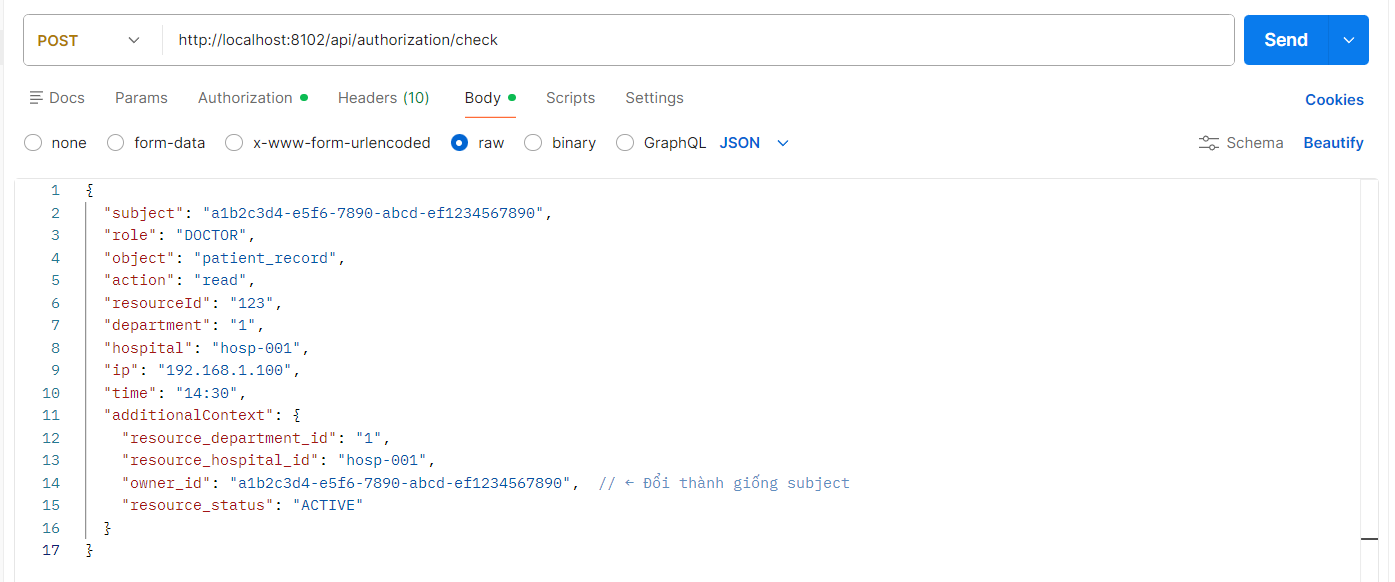
\includegraphics[width=1\linewidth]{images/request.png}
    \caption{Decision Request - Doctor reads patient record}
    \label{fig:request}
\end{figure}


The PDP returns a response that the gateway can enforce immediately. The response includes the final decision and may include a reason and the matched policy identifier for debugging and auditing. Figure~4.2 shows an example response.

\begin{figure}[H]
    \centering
    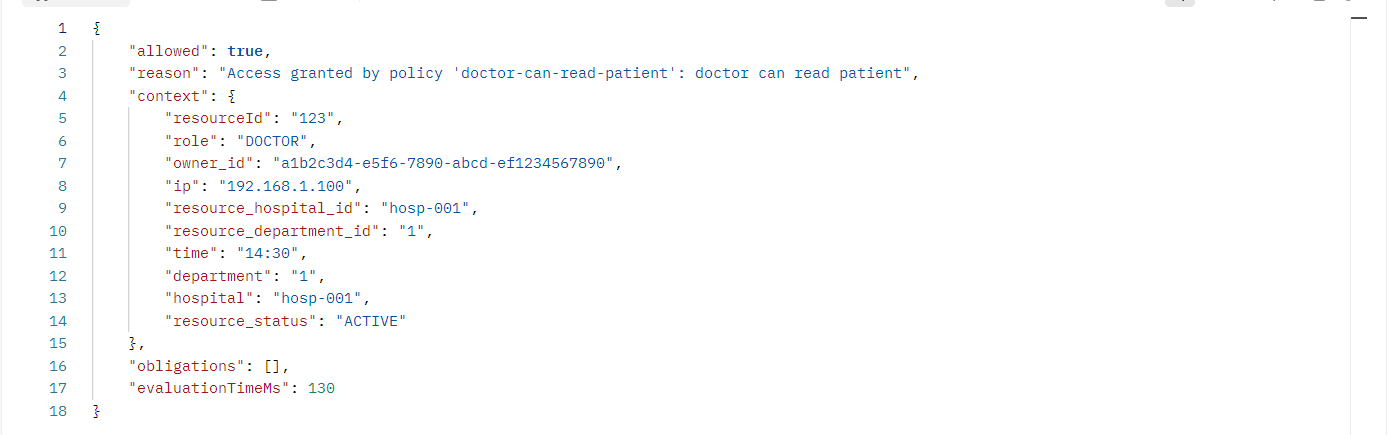
\includegraphics[width=1\linewidth]{images/response.png}
    \caption{Decision Response - Doctor reads patient record}
    \label{fig:response}
\end{figure}


\subsection{Role-centric RBAC–ABAC evaluation logic}
The PDP evaluates access in two steps. First, it checks whether the user's role grants the requested action on the resource type (RBAC baseline). Second, it evaluates attribute-based constraints (ABAC) to narrow access based on context and resource attributes. A request is permitted only if both steps succeed.
\vspace{0.5cm}


The baseline RBAC check prevents policies from granting access outside the role definition. In other words, attributes in this design are used to restrict access, not to expand it beyond the RBAC permission set.
\begin{figure}[H]
    \centering
    \small
    \begin{lstlisting}]
function decide(req):
    assert req.action, req.subject, req.object

  # Step 1: RBAC baseline (role -> permission)
  if not rbac_allows(req.subject.roles, req.action, req.object):
    return DENY("RBAC baseline denied")

  # Step 2: attribute enrichment (PIP)
  attrs = pip_get_attributes(req.subject.keycloak_user_id, req.object, req.resourceId)

  # Step 3: ABAC constraints (OPA)
  opa_input = build_opa_input(req, attrs)  # maps to input.resource.object/action for Rego
  if not opa_allows(opa_input):
    return DENY("ABAC constraints denied")

  return PERMIT("RBAC+ABAC passed")
\end{lstlisting}
    \caption{PDP evaluation flow (pseudo-code)}
    \label{lsting:pseudo-code}
\end{figure}


\subsection{ Attribute retrieval via PIP}
JWT claims provide only basic identity information. Many hospital decisions require extra attributes, such as department, assignment, or patient context. For this reason, the PDP retrieves additional attributes using the Attribute Provider (PIP).

In the application, the PIP collects attributes from two sources:

\begin{itemize}
  \item \textbf{Staff attributes:} obtained from the User Service (e.g., department id, position, staff status).
  \item \textbf{Resource/context attributes:} obtained from domain services such as Patient and Appointment (e.g. sensitivity level, owner id, department,  hospital id).
\end{itemize}

\begin{figure}[H]
    \centering
    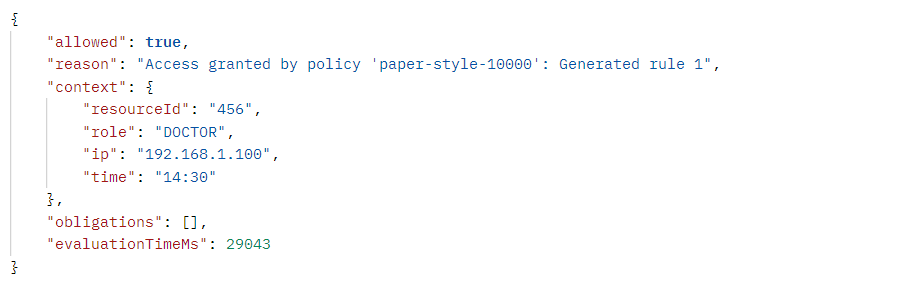
\includegraphics[width=1\linewidth]{images/attributeretrival.png}
    \caption{Attribute Retrieval}
    \label{fig:attributeretrieval}
\end{figure}

The PIP returns a compact attribute bundle. It does not return full business payloads (for example, it does not return the full Patient record content). This reduces data exposure and keeps the PIP focused on decision support.

\subsubsection{Attribute model and attribute selection}
In theory, the HMS exposes many possible attributes at the user, resource, and environment level. However,
not all of them are equally useful for access control. In the hybrid RBAC--ABAC design of this thesis, the
attribute model focuses on a small set of attributes that (i) clearly reduce RBAC over-permission in typical
hospital workflows, (ii) are available and verifiable in the microservices, and (iii) avoid unnecessary
exposure of detailed clinical data.

Conceptually, attributes are organized into three groups:

\begin{itemize}
  \item \textbf{Subject attributes} (user/staff): organizational and employment fields such as
  hospital id, department id, position level, and active status. These refine broad roles (e.g. DOCTOR,
  NURSE) into ``doctor of hospital H, department D, with at least level L, currently active''.

  \item \textbf{Resource attributes} (patient record, appointment, lab order, prescription, etc): context
  about the clinical object, including the resource hospital/department, treatment relationship
  (assigned doctor/owner), and lifecycle status (e.g. appointment status or discharge state). These
  attributes express who the record belongs to and in which department and state it is handled.

  \item \textbf{Environment/context attributes}: dynamic context such as time-of-day and shift
  (working hours flag), network zone (IP range). These attributes capture
  operational constraints such as on-duty access only or internal-network-only access.
\end{itemize}

Table~\ref{tab:attribute-comparison} compares the selected attribute groups with other candidates that
were not used as core attributes in the prototype.

\begin{table}[H]
\centering
\renewcommand{\arraystretch}{1.2}
\begin{tabular}{|p{2.4cm}|p{3.6cm}|p{5.1cm}|p{4.1cm}|}
\hline
\textbf{Category} & \textbf{Core attribute group} & \textbf{Main contribution in HMS} & \textbf{Examples not used as core} \\
\hline
Subject &
Hospital id, department id, position level, active status &
Refine broad roles into concrete staff context (which hospital/department the user works in,
seniority, and whether the staff member is still employed). This directly restricts RBAC permissions
by organization and employment state. &
Age, gender, nationality and other demographic fields; these are rarely the primary criteria for
authorization in common HMS workflows and may raise fairness concerns. \\
\hline
Resource &
Resource hospital/department, assigned doctor/owner, resource status (e.g. ACTIVE, DISCHARGED) &
Encode who the record belongs to, which department handles it, and in which lifecycle state it is.
This allows constraints such as ``only the assigned doctor in the same department may update an
active record''. &
Detailed diagnosis codes, lab result values, and full medical history. These attributes are highly
sensitive, harder to normalize, and more relevant to clinical decision-making than to baseline
authorization decisions. \\
\hline
Environment &
Time/shift (time range, working-hours-only), IP/network zone, ownership flag &
Capture operational context such as on-duty vs off-duty, internal vs external networK. These constraints are common in hospitals and can be enforced without accessing medical
content. &
Fine-grained GPS location, device posture (managed/unmanaged), or behavioural risk scores. These
attributes require additional infrastructure (MDM, tracking, ML) and add complexity that is outside
the scope of this prototype. \\
\hline
\end{tabular}
\caption{Comparison of attribute groups for the hybrid RBAC--ABAC model in the HMS prototype.}
\label{tab:attribute-comparison}
\end{table}

To make the comparison more concrete, the relative contribution of attribute groups can be estimated. In this prototype, resource-level attributes (department, hospital, status, treatment
relationship) are expected to contribute roughly $40\%$ of the ``control value'', subject-level attributes
around $35\%$, and environment/context attributes around $25\%$. Within these groups, four constraints
--- department/hospital matching, treatment relationship, time/shift, and resource status --- jointly
account for about $80$--$85\%$ of the effective reduction of RBAC over-permission, while network act as complementary safeguards.


\subsection{OPA integration and policy input}
\label{sec:opa-integration}

In this prototype, Open Policy Agent (OPA) is used as the policy evaluation engine. The Authorization
Service (PDP) does not hard-code business permissions. Instead, it builds a single input document and
asks OPA to evaluate the current request against the policy set.

\subsubsection{Policy deployment to OPA:}
Policies are managed in the Policy Service (PAP). When a policy is created or updated, the service
transforms the policy rules into an OPA-friendly format and publishes them to OPA as data. In the
normalized format, each rule becomes one entry in \texttt{data.dynamic\_policies}. For multi-rule
policies, the key format is \texttt{\{policyId\}\_\_\{ruleId\}} so OPA can evaluate rules individually
while still knowing their parent policy through fields such as \texttt{parent\_policy\_id} and
\texttt{combining\_algorithm}. This keeps the policy model readable in the Policy UI while making
evaluation in OPA straightforward.

\subsubsection{OPA input structure (request side):}
For each protected request, the PDP builds an OPA input map with three main parts:
\texttt{user}, \texttt{resource}, and \texttt{context}. The \texttt{user} object carries RBAC identity
(role) and subject attributes (e.g., department and hospital). The \texttt{resource} object describes
the target resource (object/type, action, resourceId) and resource-related attributes (e.g., resource
department, hospital, sensitivity, status). The \texttt{context} object contains environment data such as
time-of-day and client IP.
\vspace{0.5cm}


After OPA receives this input, it evaluates the request in a clear order. First, it matches rules by the basic target
fields (\texttt{resource.object} and \texttt{resource.action}) together with subject conditions such as the user's role.
Then it checks the ABAC constraints attached to each matched rule, for example department/hospital matching, ownership,
resource status, time window, and IP range. When more than one rule matches, OPA applies the policy’s combining behavior
and rule priority to decide which result takes effect. In this prototype, a matching Deny rule takes precedence over Allow,
so a deny rule can block access even if another rule allows it. Finally, OPA returns one decision object with
\texttt{allowed} and a short \texttt{reason} string, which is useful for debugging and for audit review.
\vspace{0.5cm}

Before building the final input, the PDP enriches missing fields through the PIP. For example, user
department/hospital is obtained from the User Service, while resource attributes (department/hospital,
sensitivity, status, owner) are obtained from the relevant domain service when a resourceId is present.
This enrichment step returns only the attributes needed for authorization, not full business payloads.

\subsubsection{Calling OPA and mapping the result:}
After the input document is built, the PDP calls OPA using the HTTP API endpoint
\texttt{/v1/data/hospital /authz/allow}. The Rego package \texttt{hospital.authz} returns a single
decision object with fields \texttt{allowed} (true/false), \texttt{reason}, and optional \texttt{obligations}.
The PDP converts this decision into the response format used by the gateway, which then enforces the
final Permit/Deny result. The same decision (including the reason) is also sent to the audit layer so
administrators can review why a request was allowed or denied.
\vspace{0.5cm}



\begin{figure}[H]
    \begin{lstlisting}
        # One decision
default decision := {"allowed": false, "reason": "No matching authorization policy", "obligations": []}

# Highest priority: Patient read own record (GET /api/patients/me) — no constraint check
decision := {"allowed": true, "reason": "Access granted: Patient can read own record (me)", "obligations": []} if {
    "PATIENT" in effective_roles
    input.resource.object == "patient_record"
    input.resource.action == "read"
    no_resource_id
}

else := {
    "allowed": false,
    "reason": sprintf("Access denied by policy '%s' (rule '%s'): %s", [
        display_policy_id(deny_hit[winner_deny_id]),
        winner_deny_id,
        deny_hit[winner_deny_id].policy_name,
    ]),
    "obligations": [],
} if { winner_deny_id }

else := {
    "allowed": true,
    "reason": sprintf("Access granted by policy '%s': %s", [
        display_policy_id(allow_hit[winner_allow_id]),
        allow_hit[winner_allow_id].policy_name,
    ]),
    "obligations": get_obligations(allow_hit[winner_allow_id]),
} if { winner_allow_id }

# -----------------------------------------------------------------------------
# 7. OUTPUT (single element set for authorization-service /v1/data/.../allow)
# -----------------------------------------------------------------------------
allow contains decision if { decision }
    \end{lstlisting}
    \caption{Calling OPA and mapping the result}
    \label{fig:opa-decision-output}
\end{figure}



Listing~\ref{fig:opa-decision-output} shows the final output rule in the \texttt{hospital.authz} package. OPA returns a decision object with three fields: \texttt{allowed}, \texttt{reason}, and \texttt{obligations}. The Authorization Service reads the first element returned from the \texttt{/v1/data/hospital/authz/allow} endpoint and maps it to the API response that the gateway can enforce.


\section{PEP at the Gateway and Request Routing}
\label{sec:gateway_pep}

In the prototype, the API gateway is the main Policy Enforcement Point (PEP). This means every external request must pass
through the gateway before it can reach any business microservice. The gateway has a clear responsibility: it does not
decide whether a request should be allowed, but it \textit{enforces} the decision returned by the PDP. This separation is
important for two reasons. First, it prevents accidental bypass, because domain services are not exposed directly to the
public network. Second, it ensures that all services follow the same enforcement logic, instead of re-implementing access
checks in each microservice.

\vspace{0.5cm}

From an implementation view, the gateway performs three steps on protected endpoints. It validates the JWT token, it
creates a decision request and calls the PDP, and it routes the request only when the outcome is Permit. If the outcome is
Deny, the gateway stops the request early and returns \texttt{403 Forbidden}. The following subsections describe these
steps in detail.

\subsection{JWT validation and claim extraction}
\label{subsec:gateway_jwt}

For each incoming request, the gateway first checks the \texttt{Authorization} header. If the header is missing, or the
token cannot be verified, the gateway returns \texttt{401 Unauthorized}. In the prototype, authentication is delegated to
Keycloak, so the gateway validates the token signature and standard fields such as issuer, audience, and expiration time.

\vspace{0.5cm}


When the token is valid, the gateway extracts a minimal set of claims that are required to build an authorization request.
This typically includes the subject identifier (user id), the role list, and optional tenant fields if they exist in the
token (for example hospital id). These fields are treated as baseline identity context, not as a complete attribute set.
The gateway does not attempt to fetch complex attributes such as department assignment or patient relationship. Those
attributes are collected later by the PDP through the PIP when required by policy constraints.

\vspace{0.5cm}


To support traceability, the gateway can generate or forward a correlation id for each request. This id is included in
logs and can be passed to the PDP and Audit Service. It helps connect a user request with its authorization decision and
domain-service execution.

\subsection{Protected endpoint interception}
\label{subsec:gateway_protected}

Not all endpoints require authorization checks. The gateway therefore distinguishes between public routes and protected
routes. Public routes include endpoints such as health checks or login-related callbacks. Protected routes include HMS
operations that access sensitive resources, such as patient records, appointments, lab results, prescriptions, and billing
data.
\vspace{0.5cm}


For protected routes, the gateway performs authorization before forwarding traffic. The core idea is simple: the gateway
does not call a business service until it receives a Permit decision. This reduces the risk of information leakage. It
also simplifies the domain services, because they can focus on business logic and assume that requests reaching them have
already passed a centralized access check.
\vspace{0.5cm}


In practice, the gateway needs a consistent way to translate an HTTP request into authorization terms. The prototype uses a
mapping from \texttt{(HTTP method, path pattern)} to \texttt{(resource type, action)}. This mapping is important because it
keeps policy writing stable. For example, reading a patient record is always evaluated as \texttt{patient\_record/read}
even if the actual URL contains many path parameters. Similarly, creating an appointment is always evaluated as
\texttt{appointment/create}. This mapping layer makes policies easier to review and reduces ambiguity.

\subsection{Decision request creation and PDP call}
\label{subsec:gateway_pdp_call}

Once the gateway confirms that a request targets a protected endpoint, it creates a decision request and calls the PDP.
The decision request is designed to be compact and consistent across all services. It contains four logical parts:
\texttt{subject}, \texttt{action}, \texttt{resource}, and \texttt{context}.
\vspace{0.5cm}


The \texttt{subject} is built from JWT claims. It includes the user identifier and the user roles. The \texttt{action} and
\texttt{resource} are built from the gateway mapping described earlier. The gateway also extracts a resource id when it is
available in the path, for example \texttt{/patients/\{patientId\}}. The \texttt{context} contains runtime metadata that can
be useful for constraints, such as request time and client IP address. The gateway keeps this context minimal and avoids
sending unnecessary user or business information to the PDP.
\vspace{0.5cm}


After building the decision request, the gateway calls the Authorization Service. If the PDP returns Permit, the gateway
routes the original request to the target microservice and returns the service response to the client. If the PDP returns
Deny, the gateway returns \texttt{403 Forbidden} and does not call the domain service. This behavior makes enforcement
explicit and consistent for all protected endpoints.
\vspace{0.5cm}


The prototype also needs a clear strategy when the PDP is unavailable. In a hospital setting, sensitive data access should
not be granted when the decision service is down. For this reason, the recommended default for protected endpoints is
\textit{fail-close}. In fail-close mode, the gateway denies the request when it cannot obtain a decision within a timeout.
The gateway logs the failure with the correlation id so that the event can be investigated. Non-sensitive routes can use a
different handling strategy if needed, but protected data access should remain conservative.
\vspace{0.5cm}


Overall, the gateway implementation provides a single enforcement point for the HMS. It ensures that authorization is
checked before any business service is reached, and it keeps routing behavior aligned with the role-centric hybrid policy
model evaluated by the PDP.
\section{User Interface}
The implementation includes a simple web UI to demonstrate end-to-end workflows. The UI is designed to reflect
different roles and their typical tasks. It does not contain authorization logic. It only displays available actions
and sends requests to the gateway. The final decision is always enforced at the gateway and PDP.


\subsection{Role-based layout and menu}
The application uses one shared layout for authenticated users and different default dashboards per role. The role comes from the session (Keycloak \texttt{realm\_access.roles} or a mapped claim). A mapping in the frontend (\texttt{DASHBOARD\_BY\_ROLE}) defines the default path for each role: admin $\to$ \texttt{/admin}, doctor $\to$ \texttt{/doctor}, nurse $\to$ \texttt{/nurse}, patient $\to$ \texttt{/patient}, pharmacist $\to$ \texttt{/pharmacist}, and so on. The sidebar menu (\texttt{Menu.tsx}) uses a \texttt{useRole} hook to read the current role and shows only items whose \texttt{visible} list includes that role. So patients see appointments and their own data; doctors and nurses see patients, appointments, lab orders, and related lists; pharmacists see prescriptions and medicines; admins see everything plus policy management and audit logs; external auditors see only the audit log page. Hiding a menu item is only for convenience; the gateway and PDP enforce access. If a user opens a URL they are not allowed to use, the API returns 403 and the UI shows an error. Table~\ref{tab:role-ui} summarises the main screens per role.

\begin{table}[H]
\centering
\begin{tabular}{|l|l|}
\hline
\textbf{Role} & \textbf{Main screens / functions} \\
\hline
Admin & Dashboard, employees, patients, appointments, lab, prescriptions, policies, audit logs \\
\hline
Doctor & Patients, appointments, lab orders/results, prescriptions (view) \\
\hline
Nurse & Patients, appointments, lab orders/results, prescriptions (view) \\
\hline
Receptionist & Appointments, scheduling, patients (limited) \\
\hline
Patient & My appointments, prescriptions, lab results \\
\hline
Lab Tech & Lab orders, lab results \\
\hline
Pharmacist & Prescriptions, medicines, inventory \\
\hline
Billing Clerk & Appointments, billing, invoices \\
\hline
External Auditor & Audit logs (read-only) \\
\hline
\end{tabular}
\caption{Main UI entry points and functions by role.}
\label{tab:role-ui}
\end{table}

\begin{figure}[H]
    \centering
    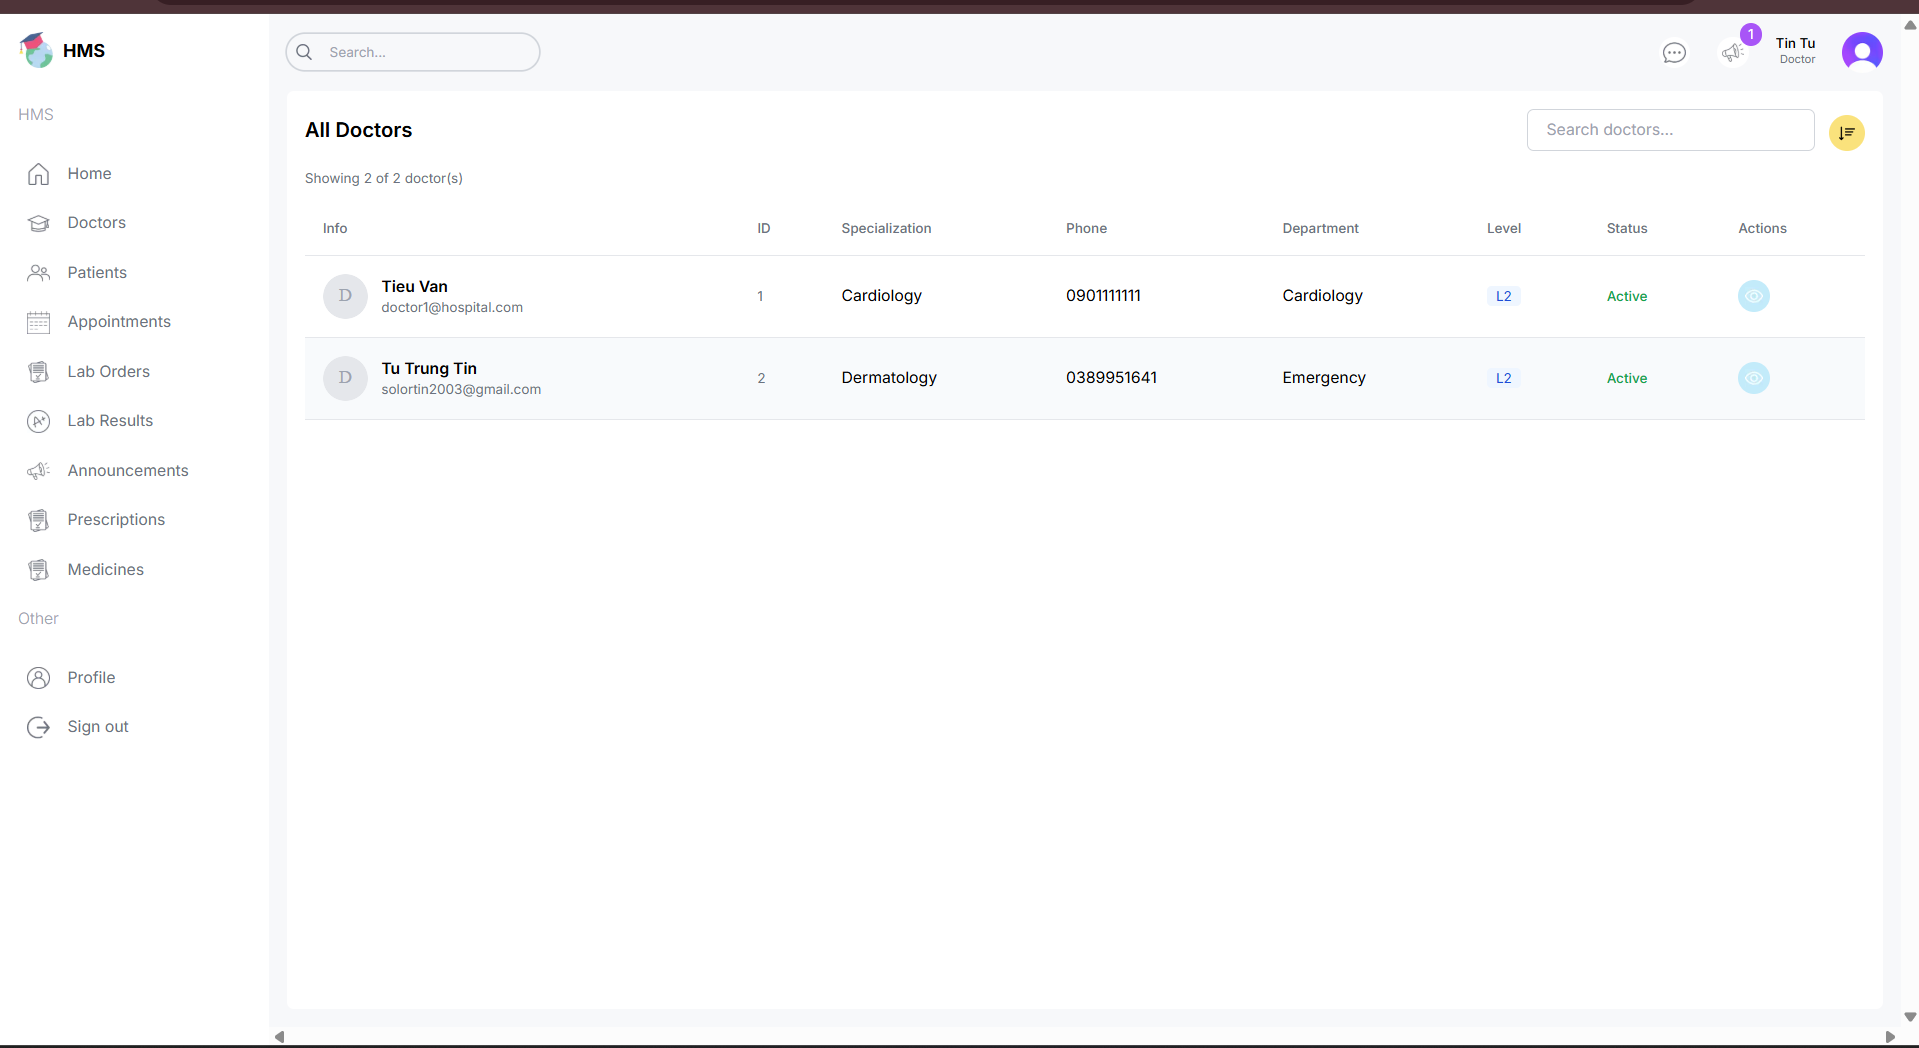
\includegraphics[width=0.75\linewidth]{images/doctorpage.png}
    \caption{Main UI for doctor role}
    \label{fig:doctorui}
\end{figure}


\begin{figure}[H]
    \centering
    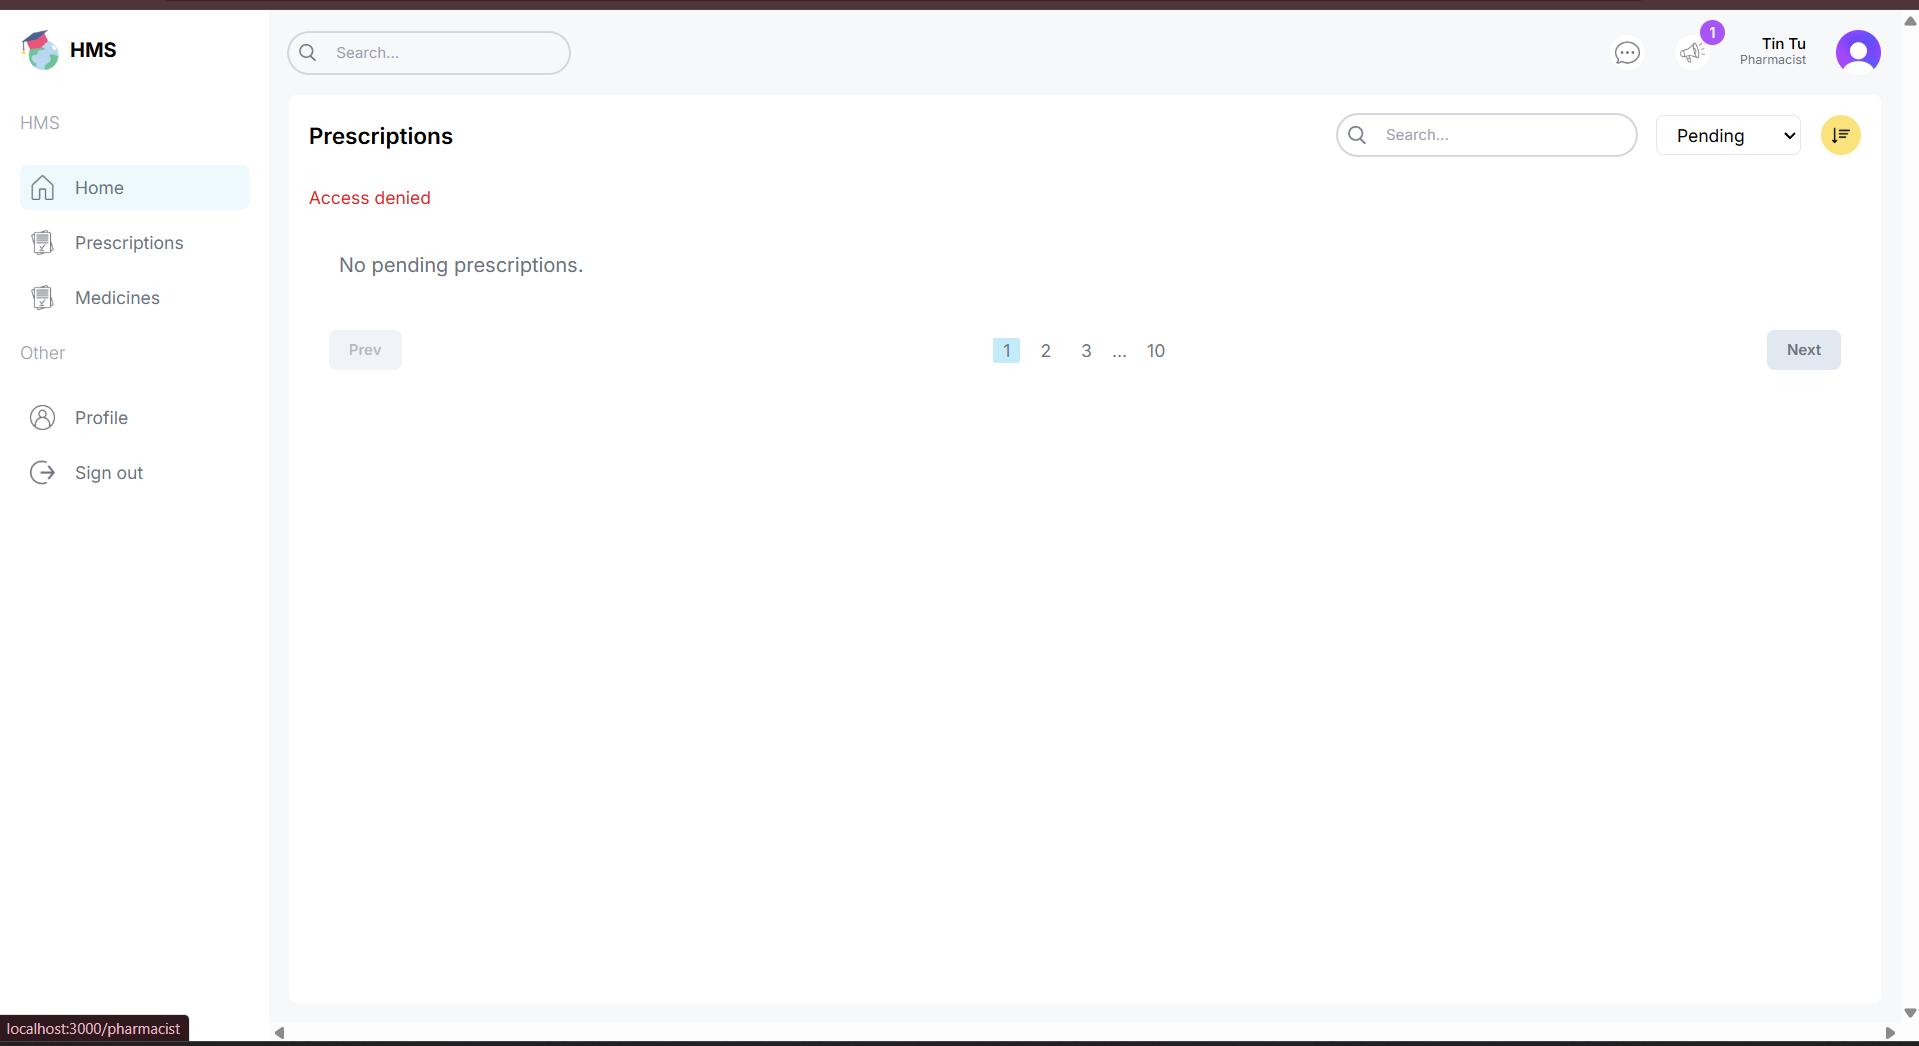
\includegraphics[width=0.75\linewidth]{images/pharmacistui.png}
    \caption{Main UI for pharmacist role}
    \label{fig:pharmacistui}
\end{figure}


\subsection{Policy Management Page}
Policy management is provided for the admin role. The goal of this UI part is to make policy operations transparent:
an admin can view existing policies, inspect the rule content, and create a new policy in a controlled format. 
\vspace{0.5cm}


Figure~\ref{fig:policymanagement} shows the policy list screen. This screen displays the policy name, status, and basic metadata so that an admin can quickly find the correct policy. From this list, the admin can open a policy to see its full content.
\begin{figure}[H]
    \centering
    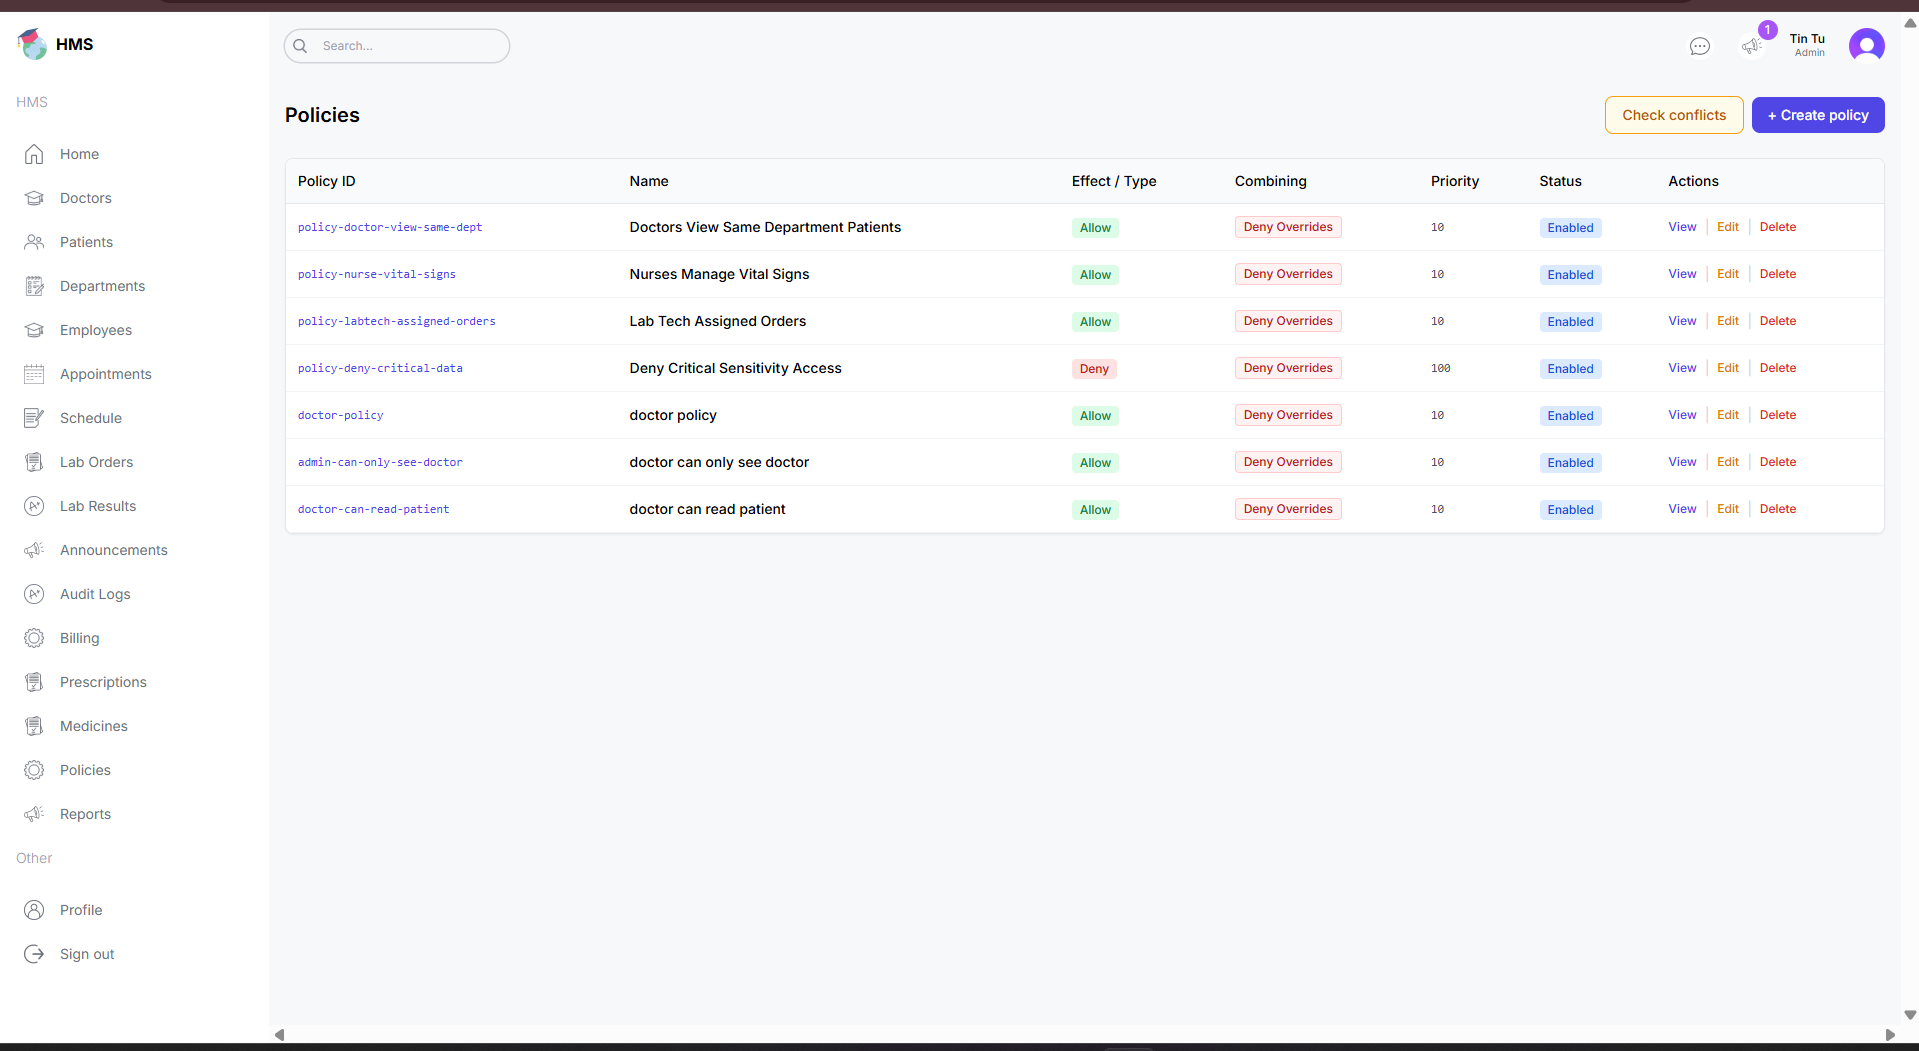
\includegraphics[width=1\linewidth]{images/policymanagement.png}
    \caption{Policy Management Page}
    \label{fig:policymanagement}
\end{figure}

Figure~\ref{fig:policydetail2} shows the policy detail screen. This view is important for review and debugging. It allows the admin to verify the target roles, resource type/object, allowed actions, effect (Allow/Deny), priority, and constraints (such as time range
or department rules). In the role-centric hybrid design of this thesis, roles define baseline access, while attributes are
mainly used as constraints to narrow access in specific contexts. This is reflected in the policy detail view, where the
role and action/resource fields are always explicit, and constraints are shown as structured conditions.

\begin{figure}[H]
    \centering
    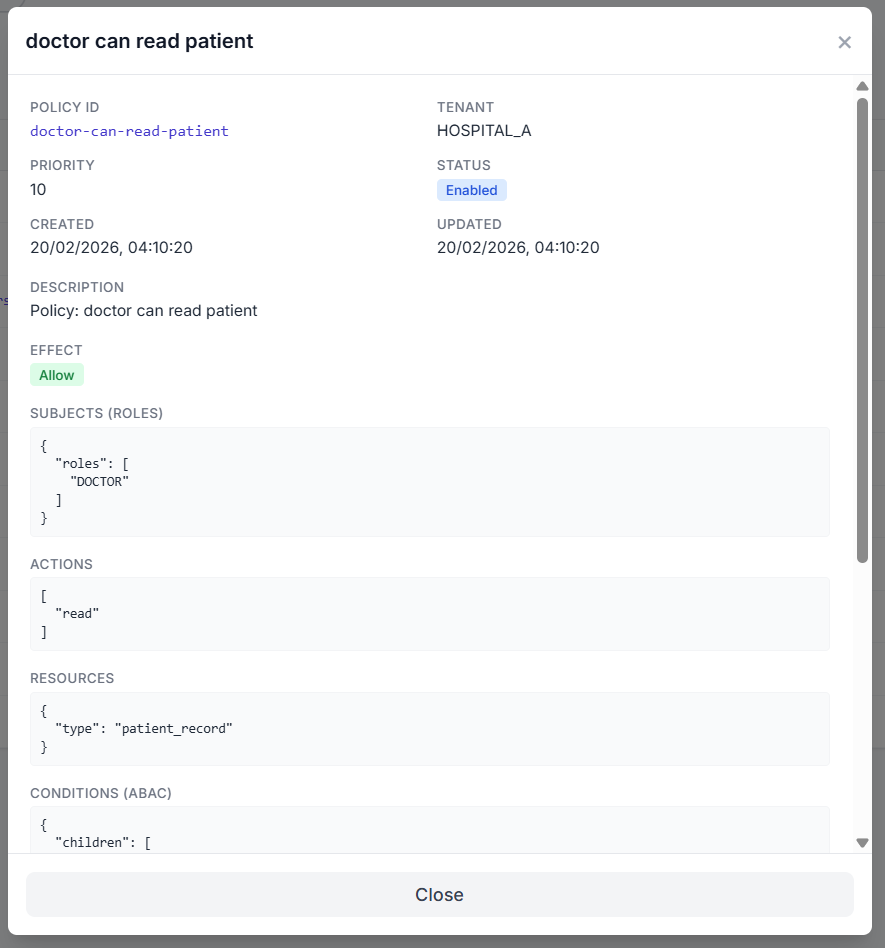
\includegraphics[width=0.65\linewidth]{images/policydetail.png}
    \label{fig:policydetail}
\end{figure}


\begin{figure}[H]
    \centering
    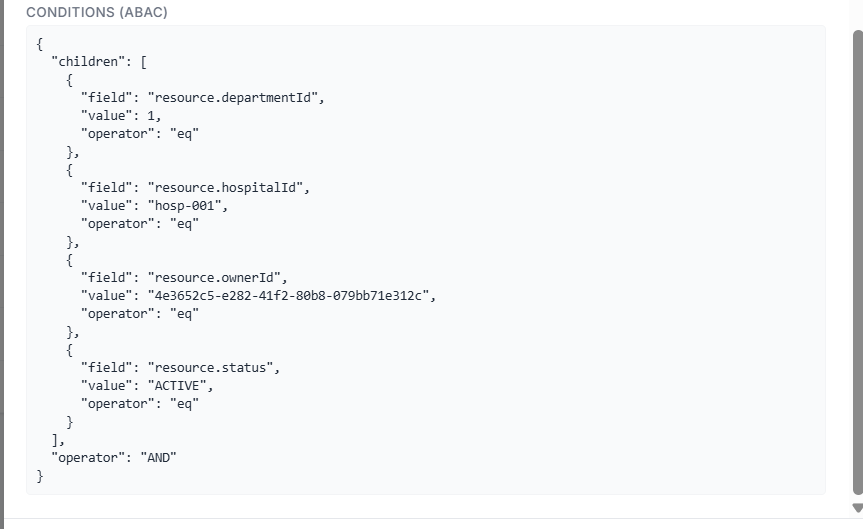
\includegraphics[width=0.65\linewidth]{images/policydetail2.png}
    \caption{Policy Detail Page}
    \label{fig:policydetail2}
\end{figure}

Figure~\ref{fig:policycreate} shows the policy creation screen. This screen is used to add a new policy or rule. In the prototype, the form is designed to reduce input errors. Fields such as action names and resource types follow a fixed naming convention so that
policies remain consistent across services. After a new policy is created, it is stored in the Policy Service database and
then published to OPA. This keeps policy authoring separate from policy evaluation.


\begin{figure}[H]
    \centering
    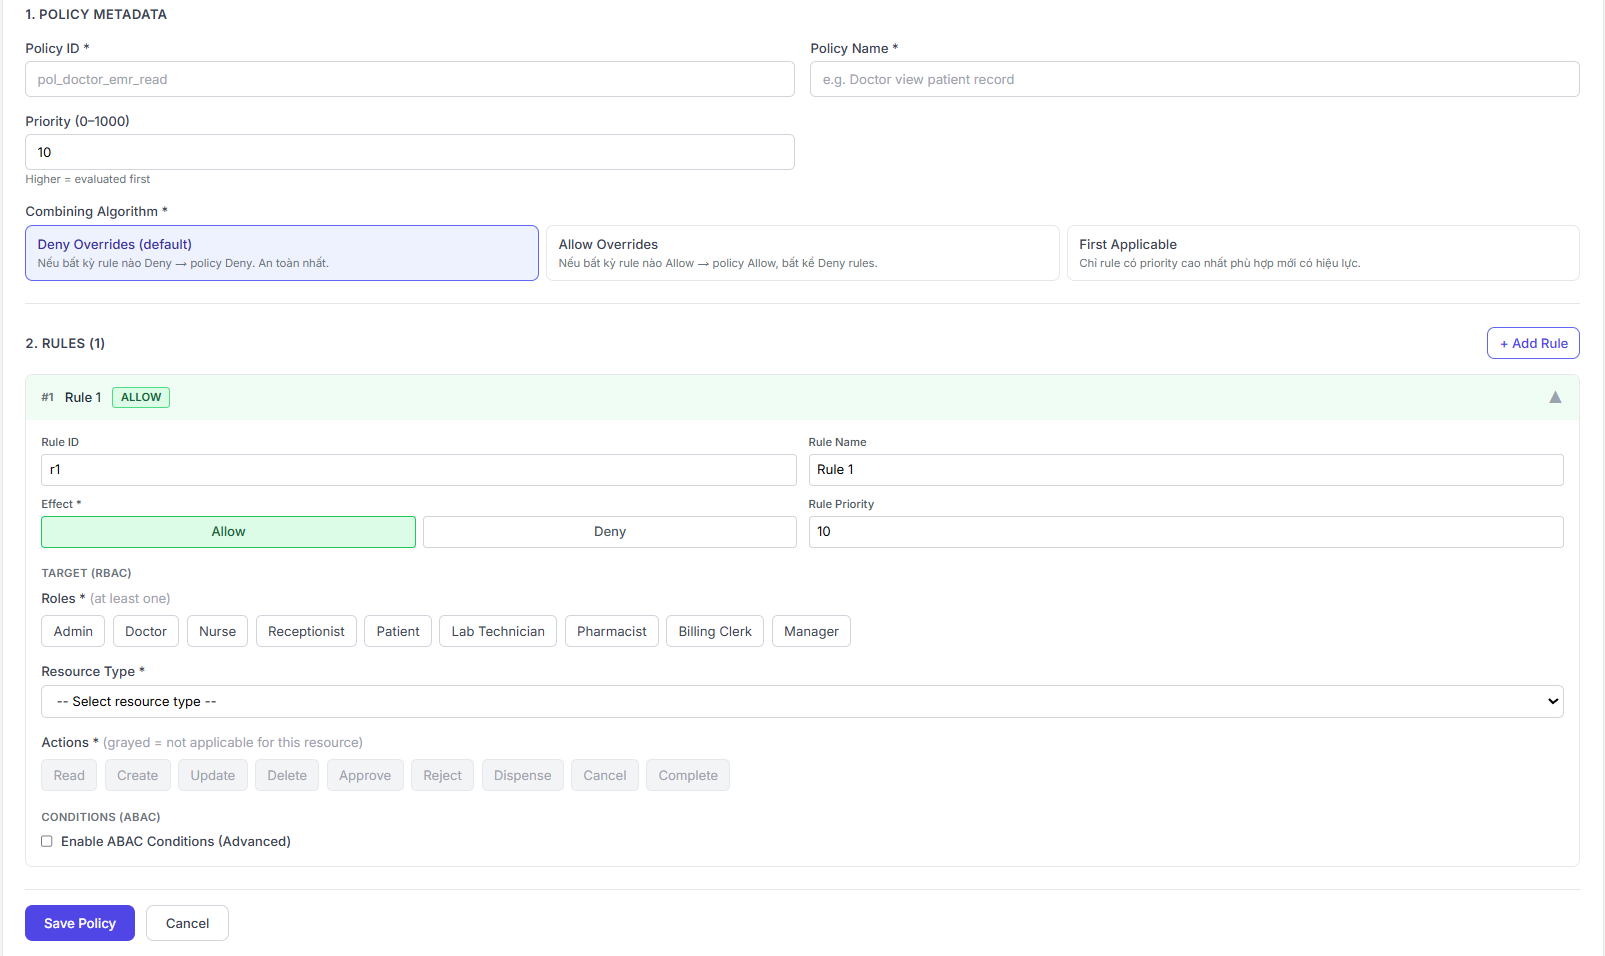
\includegraphics[width=1\linewidth]{images/polcreate.png}
    \caption{Policy create Page}
    \label{fig:policycreate}
\end{figure}





\subsection{Audit logs Page}
Audit logs are required in a hospital setting because medical data is sensitive and access must be traceable. The prototype
includes audit screens so that administrators (or authorized auditors) can review access activities and investigate abnormal
events.
\vspace{0.5cm}


Figure~\ref{fig:auditlogs} shows the audit log list screen. It provides a searchable overview of access events. A typical log entry includes the timestamp, subject identifier, role, action, resource type/object (or resource id), and the final decision (Permit/Deny).
This list view is useful for quick monitoring and for locating suspicious requests.
\begin{figure}[H]
    \centering
    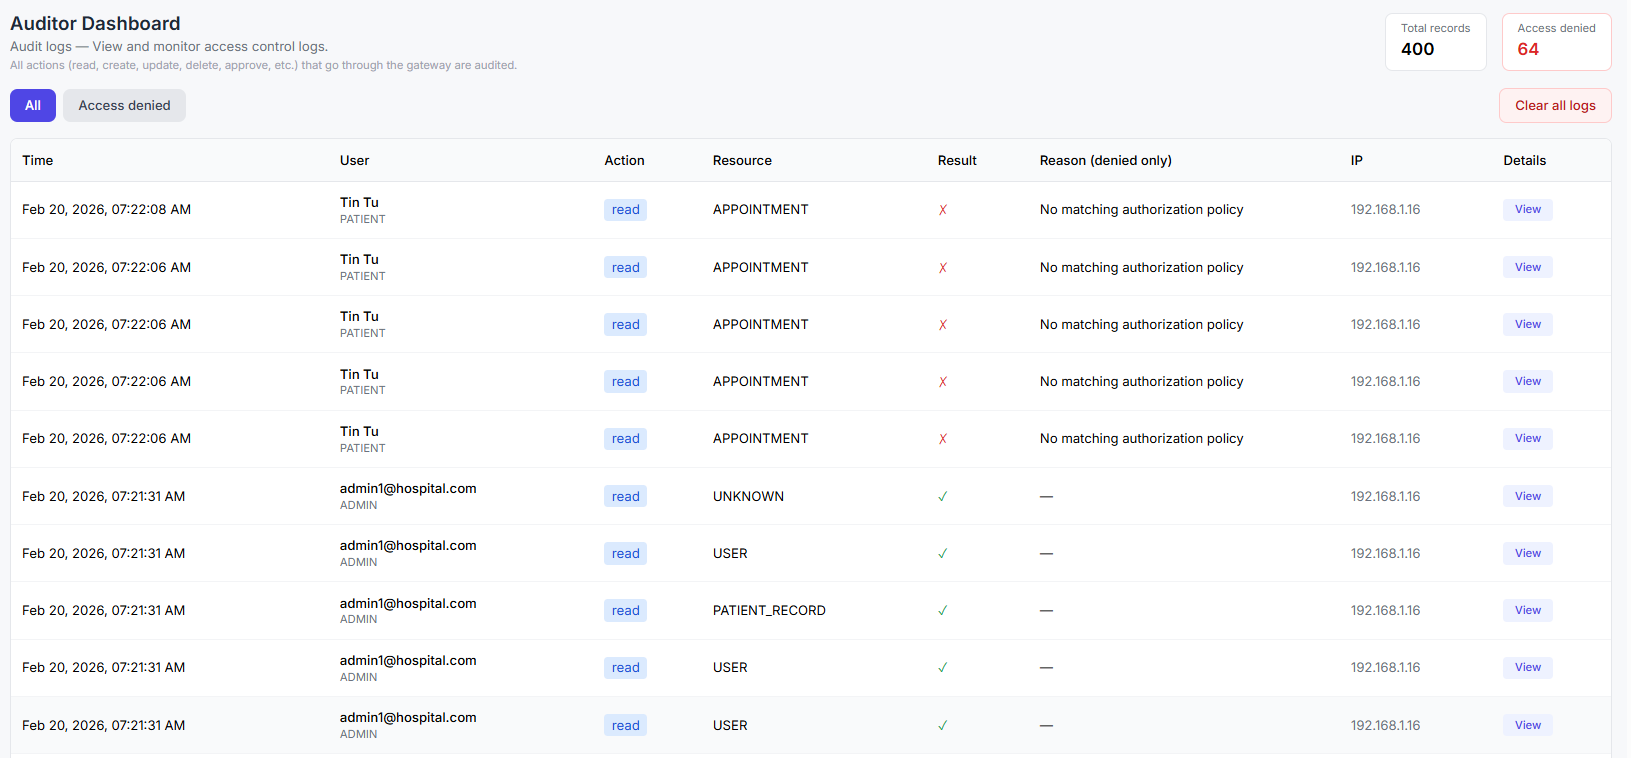
\includegraphics[width=1\linewidth]{images/auditlogs.png}
    \caption{Audit logs Page}
    \label{fig:auditlogs}
\end{figure}
Figure~\ref{fig:auditlogsdetail} shows the audit log detail screen. This screen provides more context for a specific event, such as request metadata and which policy (or rule) matched the request. This detail view is helpful when validating the correctness of policies during testing. It is also useful in real operation to support incident investigation and compliance requirements.
\begin{figure}[H]
    \centering
    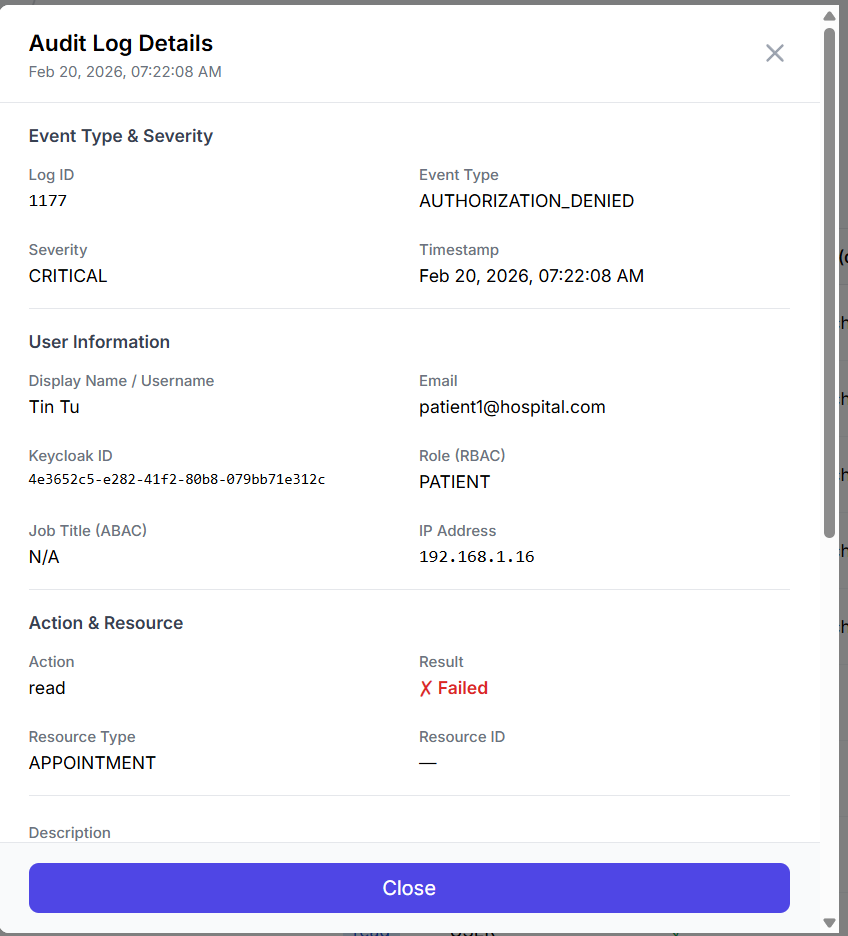
\includegraphics[width=0.55\linewidth]{images/auditlogdetail.png}
    \caption{Audit logs Detail Page}
    \label{fig:auditlogsdetail}
\end{figure}

Overall, the UI in this application serves two purposes: it demonstrates role-based workflows for HMS functions, and it provides
a practical way to manage policies and review audit trails. The next sections build on these screens to describe how policies
are evaluated and how the system can be tested and validated.

\subsection{Policy-aware navigation and access feedback}
\label{subsec:ui_policy_aware}
The UI is designed to be policy-aware at the navigation level, mainly to improve usability. After login, the UI reads the
user roles from the authentication token and shows the menus that match the role. For example, a doctor sees clinical menus
such as appointments and patient-related views, while an administrator sees policy and audit menus. This behavior reduces confusion for users and helps them focus on relevant workflows.

Hiding menu items is only a usability feature and does not enforce authorization. The final decision is always enforced by
the gateway (PEP) and the authorization layer (PDP/OPA). When a user tries to access an endpoint or page that is not
allowed, the UI provides clear feedback based on HTTP status codes:
\begin{itemize}
  \item \textbf{401 Unauthorized:} the session is missing/expired or the JWT cannot be validated. The UI prompts the user to
  sign in again.
  \item \textbf{403 Forbidden:} the user is authenticated, but the request is denied by policy. The UI shows an access
  denied message and avoids rendering sensitive data.
\end{itemize}
\begin{figure}[H]
    \centering
    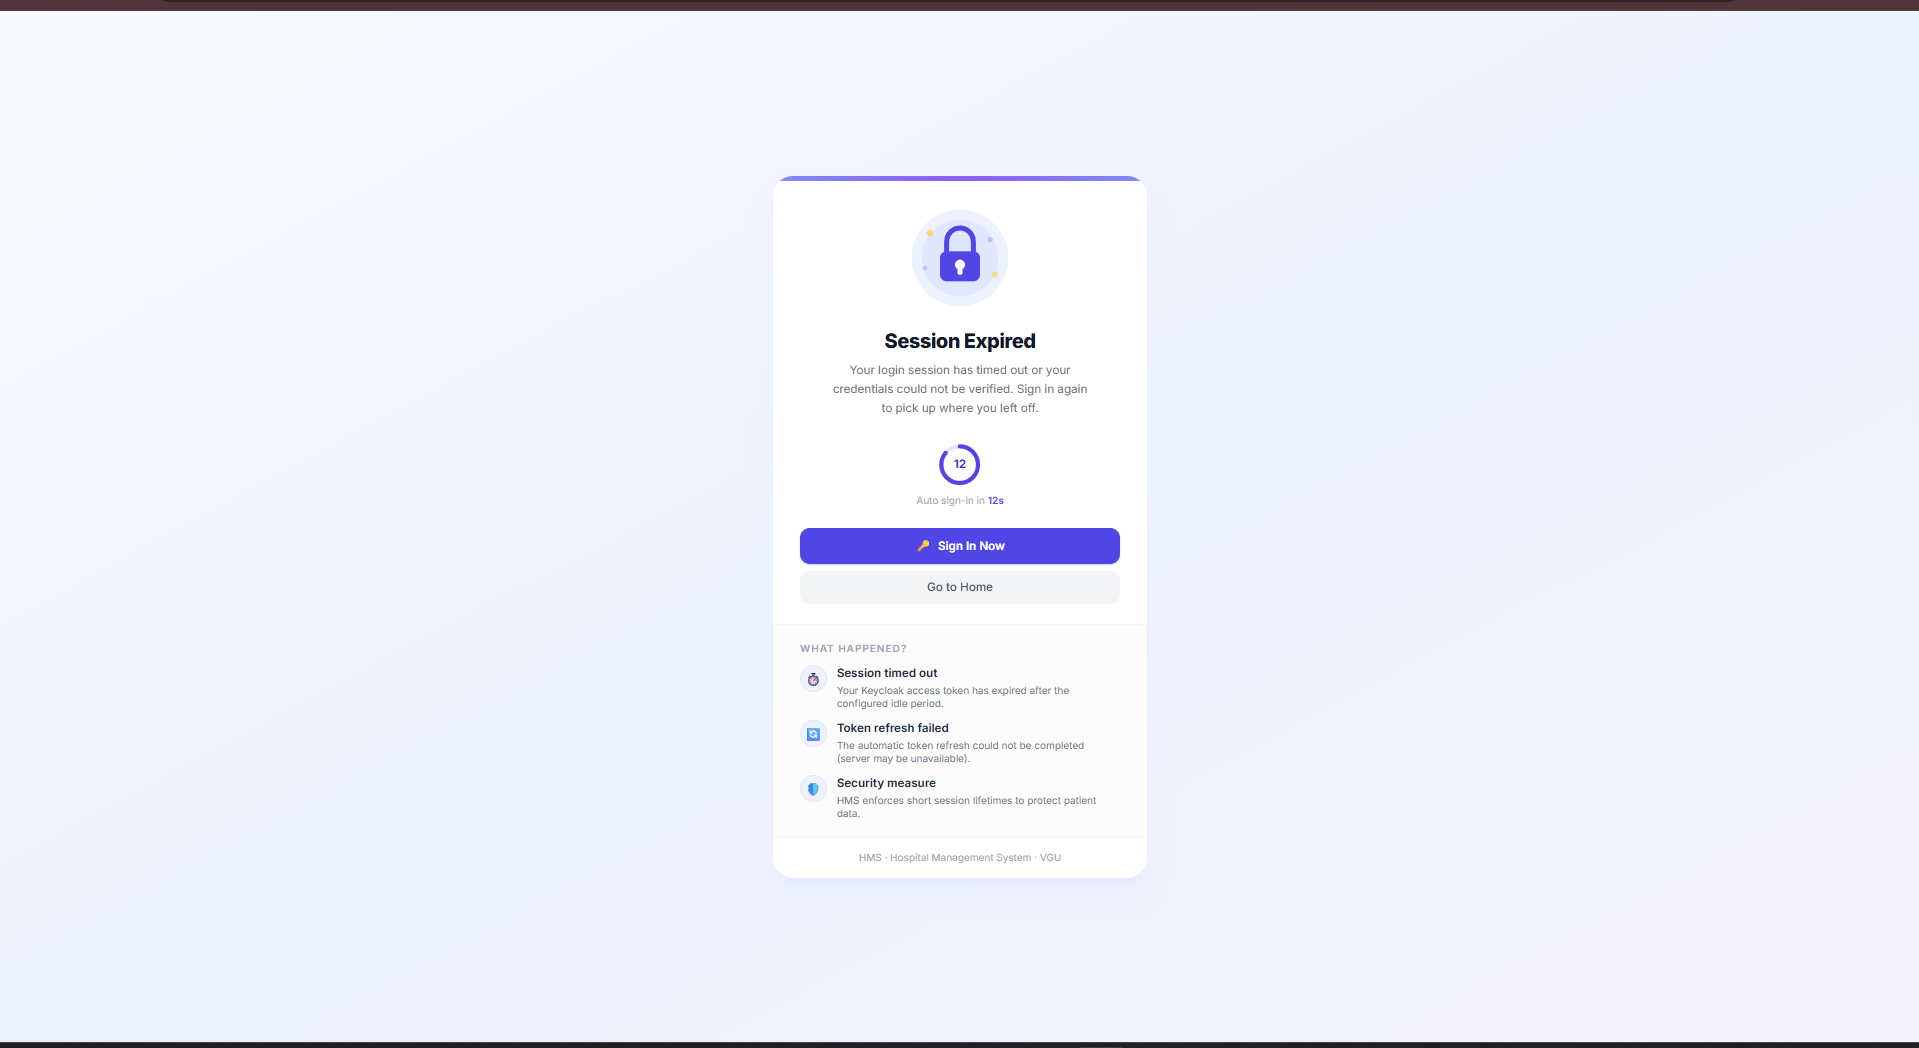
\includegraphics[width=1\linewidth]{images/ui-401-unauthorized.png}
    \caption{Policy-aware access feedback in the UI - Unauthorized, the session is missing/expired (HTTP 401)}
    \label{fig:ui-401-unauthorized}
\end{figure}


\begin{figure}[H]
    \centering
    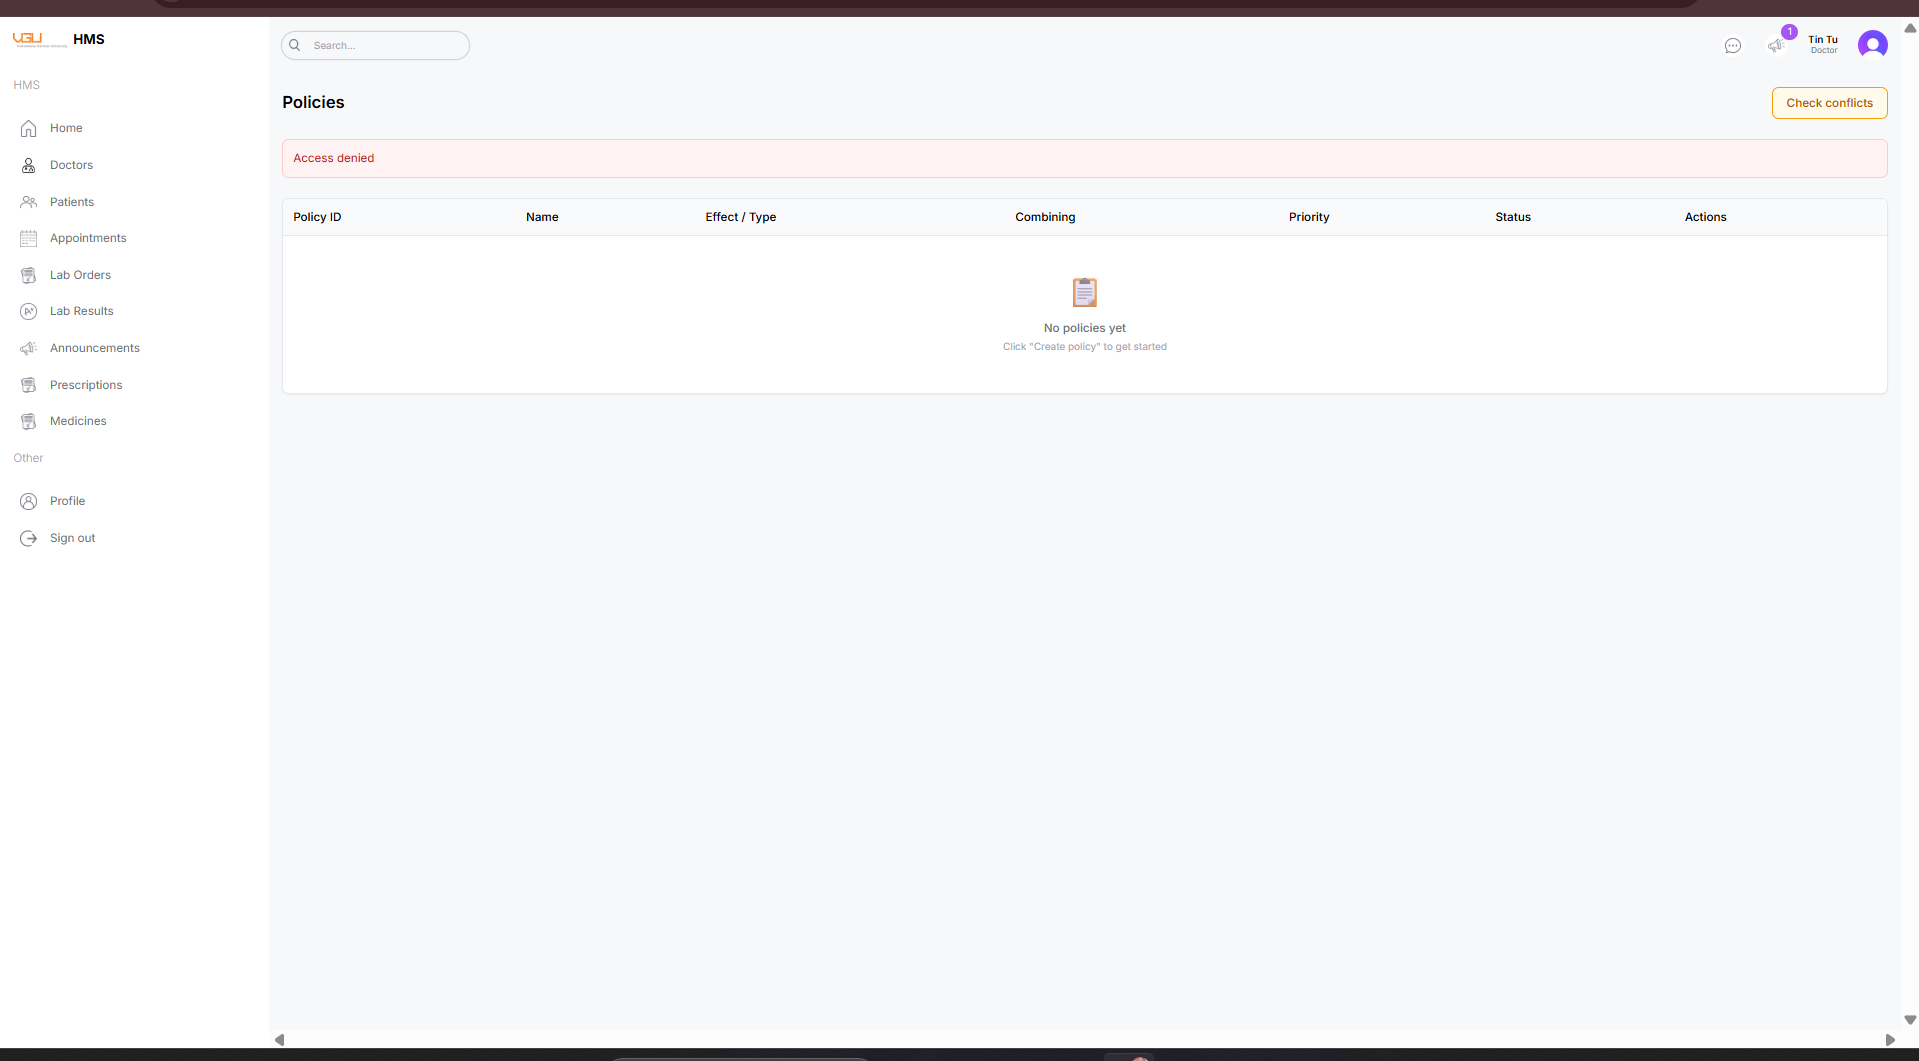
\includegraphics[width=1\linewidth]{images/ui-403-access-denied.png}
    \caption{Policy-aware access feedback in the UI - Authenticated but denied by policy (HTTP 403)}
    \label{fig:ui-403-access-denied}
\end{figure}




\section{Policy Conflict Detection Implementation}
\label{sec:policy-conflict-detection-2}

Policy conflict detection is implemented in the policy service. Its job is to find pairs of rules that can contradict each other or overlap in a way that makes the final decision unclear. The idea follows the design in Section~\ref{sec:policy-conflict-detection}: we do static analysis on the rules stored in the policy service, without running real requests. The result is a list of conflict pairs that the admin can review and fix (e.g. by merging rules, changing effects, or removing one of them).


\subsection{When detection runs and what it returns}

Detection can run in two ways. First, the admin can trigger it from the policy management page: after loading the list of policies, they click ``Check conflicts'' and the frontend calls the gateway, which forwards the request to the policy service. Second, the policy service exposes two REST endpoints. \texttt{GET /api/policies/conflicts} runs detection on all enabled policies and returns a single result. \texttt{POST /api/policies/conflicts/detect} accepts a body \texttt{\{ "policyIds": ["id1", "id2", ...] \}} and runs detection only on those policies. Both endpoints return the same shape: \texttt{totalPolicies} (number of rules considered after expanding each policy into its rules), \texttt{conflictCount}, \texttt{conflicts} (a list of conflict pairs), and \texttt{detectionTimeMs}. The frontend shows this in a panel: if \texttt{conflictCount} is 0 it shows ``No policy conflicts''; otherwise it lists each pair with the conflict type (e.g.\ \texttt{AUTH\_CONFLICT} or \texttt{REDUNDANCY\_CONFLICT}), the resource type, the overlapping actions, the reason text, and when available a witness (a sample attribute map that matches both rules). Figure~\ref{fig:policyconflitdetection} shows a real run: 11 policies scanned in 36\,ms with one redundancy conflict between \texttt{doctor-policy\_r1} and \texttt{admin-create-patient\_r1} on resource \texttt{patient\_record} for actions read, create, update, with witness \texttt{\{"roles":"ADMIN", "type":"patient\_record"\}}. 


\begin{figure}[H]
    \centering
    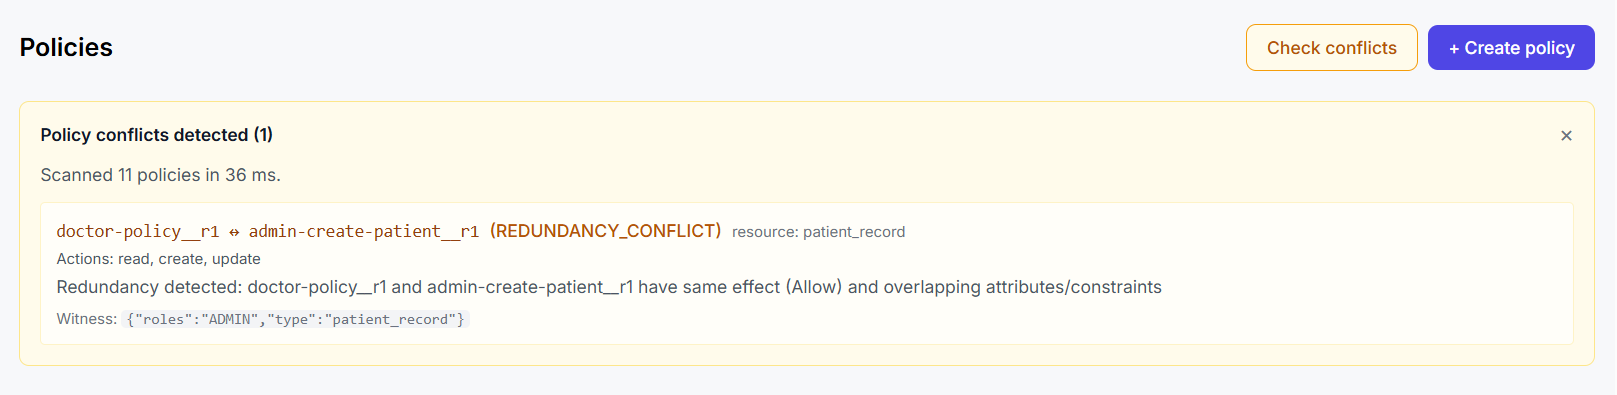
\includegraphics[width=1\linewidth]{images/policyconflict.png}
    \caption{Policy Conflict Detection Result}
    \label{fig:policyconflitdetection}
\end{figure}

\subsection{Types of conflicts}

The implementation detects two kinds of conflicts:
\begin{itemize}
    \item \textbf{Authorization conflict (Allow vs Deny).} Two rules conflict in this sense if one has effect Allow and the other Deny, and there exists at least one request that would match both rules. So we require: (1) the two rules have different effects; (2) their action sets overlap (e.g. both include \texttt{read}); (3) they apply to the same resource type (or one of them does not restrict resource type); (4) for each attribute that both rules use (subject or resource), the value sets intersect (e.g. one says role in \texttt{\{DOCTOR\}} and the other says role in \texttt{\{DOCTOR, NURSE\}}); and (5) if both rules have a time-range constraint, those intervals overlap. When all these hold, we report an \texttt{AUTH\_CONFLICT} and include the overlapping actions and a short reason (e.g. which two policies and that they have conflicting effects for those actions).
    \item \textbf{Redundancy.} Two rules are redundant if they have the same effect (both Allow or both Deny) and again there is some request that matches both. So the conditions are the same as above except the effects must be equal. In that case we report \texttt{REDUNDANCY} (or \texttt{REDUNDANCY\_CONFLICT} in the code). The admin may want to remove one of the rules or merge them to keep the policy set simpler.
\end{itemize}


Each conflict pair in the result includes the two rule identifiers (policy id and rule id), the conflict type, the list of overlapping actions, and a \texttt{reason} string. Optionally a \texttt{witness} (or \texttt{witnessRequest}) is provided: a sample attribute-to-value map that would satisfy both rules, which helps when debugging.

\subsection{How the algorithm works}

The service loads all enabled policies (or only the ones requested in the POST body), then expands each policy into a list of rules. Each rule has subject attributes (e.g. role, department), resource type, actions, and optionally object attributes and conditions (e.g. time range). Rules that have no actions or no subject/resource attributes are skipped; they cannot participate in a conflict in our definition.
\vspace{0.5cm}


To avoid comparing every pair of rules (which would be too slow with many policies), the code does a few things. First, rules are grouped by resource type. Within each group, rules are split into Allow and Deny. Only Allow--Deny pairs need to be checked for authorization conflicts; within the same effect we only check for redundancy. Second, within each resource-type bucket, rules are indexed by action: for each action we keep a list of rule indices. So we only compare an Allow rule and a Deny rule if they share at least one action. That cuts down the number of pairs a lot. Third, for rules that have a time-range constraint, the code builds a list of disjoint time intervals (using \texttt{TimeIntervalReducer}) and uses binary search (\texttt{TimeIntervalBinarySearch}) to find which rules overlap in time. So we do not need to compare every Allow with every Deny when many rules have time constraints; we only compare when the time intervals overlap.
\vspace{0.5cm}


For each candidate pair (Allow, Deny) or (same-effect, same-effect), the code checks attribute overlap. Subject attributes and object (resource) attributes are compared: for each attribute that appears in both rules, we check whether the value sets intersect (e.g. \texttt{\{DOCTOR\}} and \texttt{\{DOCTOR, NURSE\}} intersect). If one rule uses attributes that the other does not have, we still need some overlap on the shared attributes; the exact logic (full overlap vs partial) is what distinguishes conflict types like exception vs association in the literature; here we report either \texttt{AUTH\_CONFLICT} or \texttt{REDUNDANCY} with a reason string.
\vspace{0.5cm}

\subsection{Policy governance and misuse prevention (implementation)}
\label{sec:governance-implementation}
Section~\ref{sec:policy-governance} (Chapter~3) defines governance controls to prevent conflicts and abuse of power in the hybrid system. This subsection describes how they are implemented and demonstrated in the prototype, so that the design is not only stated but \emph{solved} from theory to demo.
\vspace{0.5cm}

\paragraph{Conflict-on-save (enforcing conflict-freedom).}
The policy service is configured with \texttt{policy.conflict-on-save: strict} in the main deployment. On create or update, the service runs conflict detection on the proposed state (all enabled policies plus the new or updated one). If any AUTH\_CONFLICT is found, the save is rejected with HTTP 409 and a conflict report is returned (policy id, rule ids, overlapping actions, reason). The UI displays this report so the administrator can resolve the conflict before retrying. Thus the invariant that the enabled policy set is conflict-free is maintained at every successful save.
\vspace{0.5cm}

\paragraph{Restricted policy administration (enforcing write-restriction).}
Policy write operations (create, update, delete policies; trigger OPA sync; run conflict detection) are protected by \texttt{@PreAuthorize("hasRole('ADMIN')")} in the policy service and by gateway route rules that allow only the ADMIN role for \texttt{/api/policies} write endpoints. A non-admin user who attempts to create or update a policy receives HTTP 403 Forbidden. This enforces the write-restriction invariant and prevents abuse by non-privileged users.
\vspace{0.5cm}

\paragraph{Traceability.}
Each policy record stores \texttt{version}, \texttt{created\_at}, \texttt{updated\_at}, \texttt{created\_by\_keycloak\_id}, and \texttt{updated\_by\_keycloak\_id}. This provides who-changed-what-when for every policy change and supports accountability. Optionally, policy create/update events can be published to the audit service so that privileged operations appear in the audit log; the prototype's audit path already records authorization decisions and can be extended to include policy lifecycle events.
\vspace{0.5cm}

\paragraph{Demo scenarios for governance.}
To show that conflict and abuse are actively prevented, the following scenarios can be demonstrated: (1) \textbf{Conflict prevention:} add or edit a policy so that a new rule conflicts (Allow vs Deny) with an existing rule for the same action and resource; the API returns 409 and the UI shows the conflict report; the policy set is unchanged. (2) \textbf{Abuse prevention:} call the policy create or update endpoint with a user that has a non-admin role (e.g.\ DOCTOR); the gateway or policy service returns 403. (3) \textbf{Traceability:} after an admin updates a policy, inspect the policy record or audit log to see the new version, timestamp, and \texttt{updated\_by} identity. These scenarios link Section~\ref{sec:policy-governance} to the running system and show that the hybrid implementation is effectively controlled.
\vspace{0.5cm}

\section{Evaluation}
\label{sec:evaluation}

This section evaluates the prototype with two goals. First, it validates authorization correctness using scenario-based test
cases, ensuring that the gateway enforces Permit/Deny decisions as defined by the role-centric hybrid policy set. Second, it
evaluates policy conflict detection as the main focus, including the correctness of conflict reports and the scalability of
conflict checking time as the number of policies grows.

\subsection{Scenario-based correctness validation}
Authorization correctness is validated using scenario-based test cases derived from the main workflows described in
Chapter~3. Each scenario defines a role, an API request sent through the gateway, the corresponding resource/action
mapping, the key constraints (such as department matching, ownership, time window, or resource status), and an expected
decision (Permit or Deny). The system is considered correct for a scenario if the gateway enforces the expected outcome:
a permitted request is forwarded to the target service successfully, while a denied request is blocked at the gateway and
returns \texttt{403 Forbidden}. Evidence is recorded using the HTTP response status together with a correlation identifier
(\texttt{X-Request-Id}) that can be used to locate the corresponding audit record.
\vspace{0.5cm}


Table~\ref{tab:scenario_test_matrix} summarizes the scenario-based test matrix. In total, \texttt{5} scenarios were
executed. The prototype produced the expected decision in \texttt{5} scenarios, resulting in an overall pass rate of
\texttt{100}\%. No unexpected Permit decisions were observed in the tested cases. For denied scenarios, the gateway returned
\texttt{403 Forbidden} consistently, which confirms that enforcement is performed before requests reach the business services.


\begin{table}[H]
\centering
\small
\begin{tabular}{|p{0.9cm}|p{2.4cm}|p{3.2cm}|p{2.8cm}|p{4.7cm}|p{1.2cm}|}
\hline
\textbf{ID} & \textbf{Role / User} & \textbf{API request } & \textbf{Resource / Action} & \textbf{Key constraints / context} & \textbf{Result} \\
\hline

1 & Doctor &
\texttt{GET /patients/ \{patientId\}} &
\texttt{patient\_record / read} &
Same hospital; doctor department matches patient department (or the doctor is assigned to this patient). &
Permit \\
\hline

2 & Doctor &
\texttt{GET /patients/ \{patientId\}} &
\texttt{patient\_record / read} &
Different department and not assigned to the patient (context violates department/assignment constraint). &
Deny \\
\hline

3 & Nurse &
\texttt{PATCH /patients/ \{patientId\}/ vitals} &
\texttt{patient\_record / update} &
Same ward/department and shift time is valid; update allowed only for vitals (scope-limited update). &
Permit \\
\hline

4 & Receptionist &
\texttt{POST /appointments} &
\texttt{appointment / create} &
Same hospital; appointment creation allowed; does not require clinical-data permission. &
Permit \\
\hline

5 & Receptionist &
\texttt{GET /patients/ \{patientId\}} &
\texttt{patient\_record / read} &
Receptionist role has no baseline permission to read medical record (RBAC baseline fails). &
Deny \\
\hline

\end{tabular}
\caption{Scenario-based test matrix for authorization correctness}
\label{tab:scenario_test_matrix}
\end{table}

The results also show the intended behavior of the role-centric hybrid model. First, scenarios where the RBAC baseline does
not grant an action (for example, a receptionist attempting to read a patient medical record) were denied immediately. This
confirms that ABAC constraints do not expand access beyond what the role allows. Second, scenarios where the RBAC baseline
permits the action but ABAC constraints fail (for example, wrong department, invalid resource status, or outside the allowed
time window) were also denied. These cases demonstrate the main advantage of the hybrid design: the system can narrow access
based on context while keeping the baseline permission model readable. Finally, scenarios where both the RBAC baseline and
ABAC constraints hold were permitted and completed successfully.
\vspace{0.5cm}


For all executed scenarios, an audit record was generated with the correlation identifier and the final decision. This
supports traceability and makes it possible to review why a request was permitted or denied during later analysis.



\subsection{ Conflict detection performance}
To evaluate the scalability of the conflict detection algorithm, we conducted performance tests with varying rule counts. The tests measure detection time and conflict counts for policy sets ranging from 1,000 to 10,000 rules. Table~\ref{tab:conflict-detection-performance} presents the results.

\begin{table}[H]
\centering
\begin{tabularx}{\textwidth}{|l|r|X|}
\hline
\textbf{Rule Count} & \textbf{Detection Time (ms)} & \textbf{Conflicts Found} \\
\hline
1000 & 493 & 18,638 \\
\hline
3000 & 2,218 & 171,538 \\
\hline
5000 & 3,309 & 479,278   \\
\hline
10000 & 18,751 & 1,890,378  \\
\hline
\end{tabularx}
\caption{Conflict Detection Performance: Detection Time vs Rule Count (1 rule per policy). Synthetic workload with overlapping subject/action/resource.}
\label{tab:conflict-detection-performance}
\medskip
\raggedright
\footnotesize
\textit{Note.} Workload: 50\% Allow / 50\% Deny; limited action/role/resource sets so many pairs overlap (synthetic stress). In practice, conflict counts are usually much lower after policy curation. Detection time includes full scan and reporting of all conflict pairs.
\end{table}

\subsubsection{Analysis of Results}

The results show the expected trend: detection time increases as the number of rules grows. For 1,000 rules, detection completes in 493\,ms, while 10,000 rules require 18.7\,s. The increase is not purely quadratic in this workload because the implementation reduces the comparison space using resource-type bucketing and action indexing (Section~\ref{sec:policy-conflict-detection}). At the same time, the runtime also depends on how many overlaps exist and how many conflicts must be reported.


The synthetic workload used in these tests intentionally creates many overlapping rules (50\% Allow / 50\% Deny, with limited action/role/resource sets) to stress-test the algorithm. As a result, the conflict counts are high (e.g., 1.89 million conflicts for 10,000 rules). In practice, after policy curation and conflict resolution, conflict counts are typically much lower, and detection time would be correspondingly faster.

\subsubsection{Scalability Characteristics}

The algorithm's scalability comes from three optimizations:

\begin{itemize}
    \item \textbf{Resource-type bucketing:} Rules are grouped by resource type, reducing the search space for each comparison.
    \item \textbf{Action indexing:} Within each resource bucket, rules are indexed by action, so only rules sharing at least one action are compared.
    \item \textbf{Time-interval optimization:} For rules with time-range constraints, binary search on disjoint intervals avoids unnecessary comparisons.
\end{itemize}

Overall, these optimizations reduce unnecessary comparisons compared to a naive all-pairs approach. In practice, the observed runtime depends on the number of rules, the amount of overlap between rules, and the amount of output generated (conflict pairs). For policy sets with thousands of rules, detection can complete within seconds in our stress test, which is acceptable for on-demand checks during policy management.

